\documentclass[11pt,a4paper]{article}

% research_paper/preamble.tex
% ============================
% Shared preamble for journal article format.

\usepackage[utf8]{inputenc}
\usepackage[T1]{fontenc}
\usepackage{amsmath,amssymb,amsfonts}
\usepackage{graphicx}
\usepackage{grffile}
\graphicspath{{figures/}{./}}
\usepackage{adjustbox}
\usepackage{booktabs}
\usepackage{multirow}
\usepackage{float}
\usepackage{subcaption}
\usepackage{geometry}
\geometry{a4paper, margin=1in}
\usepackage{hyperref}
\hypersetup{
    colorlinks=true,
    linkcolor=blue,
    citecolor=blue,
    urlcolor=blue
}
\usepackage{cite}
\usepackage{xcolor}
\usepackage{caption}
\usepackage{microtype}

\usepackage{placeins}
\usepackage{tikz}
\usepackage{tabularx}

% Include generated macros from make_numbers.py
% Auto-generated by research_paper/scripts/make_numbers.py
% DO NOT EDIT MANUALLY. All values originate from repository metric files.

\newcommand{\CDGLOBALCIHiVI}{0.08}
\newcommand{\CDGLOBALCIHiXII}{0.14}
\newcommand{\CDGLOBALCIHiXXIV}{0.17}
\newcommand{\CDGLOBALCILoVI}{0.05}
\newcommand{\CDGLOBALCILoXII}{0.09}
\newcommand{\CDGLOBALCILoXXIV}{0.11}
\newcommand{\CDGLOBALMAEVI}{0.064}
\newcommand{\CDGLOBALMAEXII}{0.115}
\newcommand{\CDGLOBALMAEXXIV}{0.140}
\newcommand{\CDGLOBALPersistVI}{0.061}
\newcommand{\CDGLOBALPersistXII}{0.112}
\newcommand{\CDGLOBALPersistXXIV}{0.152}
\newcommand{\ConvAUCCIHiVI}{0.91}
\newcommand{\ConvAUCCIHiXII}{0.92}
\newcommand{\ConvAUCCIHiXXIV}{0.90}
\newcommand{\ConvAUCCILoVI}{0.83}
\newcommand{\ConvAUCCILoXII}{0.85}
\newcommand{\ConvAUCCILoXXIV}{0.82}
\newcommand{\ConvAUCVI}{0.871}
\newcommand{\ConvAUCXII}{0.885}
\newcommand{\ConvAUCXXIV}{0.862}
\newcommand{\ConvBSSVI}{+0.0089}
\newcommand{\ConvBSSXII}{+0.1379}
\newcommand{\ConvBSSXXIV}{+0.2088}
\newcommand{\ConvECEVI}{0.0111}
\newcommand{\ConvECEXII}{0.0198}
\newcommand{\ConvECEXXIV}{0.0221}
\newcommand{\FailedTests}{0}
\newcommand{\GBMProgressionMAE}{1.465}
\newcommand{\GRUMaskedMAE}{1.475}
\newcommand{\GRUPairedCIHi}{-0.0115}
\newcommand{\GRUPairedCILo}{-0.0814}
\newcommand{\GRUPairedDelta}{-0.0450}
\newcommand{\GRUUnmaskedMAE}{1.520}
\newcommand{\LifestyleHardCapHi}{1.35}
\newcommand{\LifestyleHardCapLo}{0.85}
\newcommand{\LifestyleShrinkage}{0.5}
\newcommand{\MMSECIHiVI}{1.51}
\newcommand{\MMSECIHiXII}{1.59}
\newcommand{\MMSECIHiXXIV}{1.72}
\newcommand{\MMSECILoVI}{1.28}
\newcommand{\MMSECILoXII}{1.34}
\newcommand{\MMSECILoXXIV}{1.41}
\newcommand{\MMSEMAEVI}{1.391}
\newcommand{\MMSEMAEXII}{1.465}
\newcommand{\MMSEMAEXXIV}{1.563}
\newcommand{\MMSEPersistVI}{1.425}
\newcommand{\MMSEPersistXII}{1.603}
\newcommand{\MMSEPersistXXIV}{1.739}
\newcommand{\MMSESlopeVI}{1.781}
\newcommand{\MMSESlopeXII}{2.108}
\newcommand{\MMSESlopeXXIV}{2.408}
\newcommand{\MRITemperature}{2.0}
\newcommand{\MRIWeight}{0.20}
\newcommand{\OCRExactMatchPct}{83.3\%}
\newcommand{\OCRFuzzyMatchPct}{8.3\%}
\newcommand{\OCRMissedPct}{8.3\%}
\newcommand{\PassedTests}{40}
\newcommand{\ProgDeltaMRICIHi}{0.0193}
\newcommand{\ProgDeltaMRICILo}{-0.0425}
\newcommand{\ProgDeltaMRIMAE}{-0.0122}
\newcommand{\SkippedTests}{1}
\newcommand{\StagerDeltaCSF}{+0.0135}
\newcommand{\StagerDeltaCSFCIHi}{0.0320}
\newcommand{\StagerDeltaCSFCILo}{-0.0009}
\newcommand{\StagerDeltaEntropyCSF}{+0.0432}
\newcommand{\StagerDeltaMRI}{+0.0201}
\newcommand{\StagerDeltaMRICIHi}{0.0396}
\newcommand{\StagerDeltaMRICILo}{0.0014}
\newcommand{\StagerDeltaTFour}{+0.0267}
\newcommand{\StagerDeltaTFourCIHi}{0.0460}
\newcommand{\StagerDeltaTFourCILo}{0.0080}
\newcommand{\StagerECEFinal}{0.0192}
\newcommand{\StagerTFourAcc}{0.811}
\newcommand{\StagerTFourFCIHi}{0.824}
\newcommand{\StagerTFourFCILo}{0.769}
\newcommand{\StagerTFourFOne}{0.796}
\newcommand{\StagerTOneAcc}{0.541}
\newcommand{\StagerTOneBAcc}{0.687}
\newcommand{\StagerTOneBFCIHi}{0.689}
\newcommand{\StagerTOneBFCILo}{0.623}
\newcommand{\StagerTOneBFOne}{0.656}
\newcommand{\StagerTOneFCIHi}{0.486}
\newcommand{\StagerTOneFCILo}{0.408}
\newcommand{\StagerTOneFOne}{0.449}
\newcommand{\StagerTThreeAcc}{0.802}
\newcommand{\StagerTThreeFCIHi}{0.814}
\newcommand{\StagerTThreeFCILo}{0.756}
\newcommand{\StagerTThreeFOne}{0.785}
\newcommand{\StagerTTwoAAcc}{0.790}
\newcommand{\StagerTTwoAFCIHi}{0.800}
\newcommand{\StagerTTwoAFCILo}{0.742}
\newcommand{\StagerTTwoAFOne}{0.771}
\newcommand{\StagerTTwoBAcc}{0.804}
\newcommand{\StagerTTwoBFCIHi}{0.817}
\newcommand{\StagerTTwoBFCILo}{0.759}
\newcommand{\StagerTTwoBFOne}{0.788}
\newcommand{\TOTSCOREMAEVI}{2.989}
\newcommand{\TOTSCOREMAEXII}{3.095}
\newcommand{\TOTSCOREMAEXXIV}{3.292}
\newcommand{\TOTSCOREPersistVI}{2.928}
\newcommand{\TOTSCOREPersistXII}{3.224}
\newcommand{\TOTSCOREPersistXXIV}{3.665}
\newcommand{\TestPct}{15.0\%}
\newcommand{\TestSubjects}{456}
\newcommand{\TotalRows}{22,168}
\newcommand{\TotalSubjects}{3,034}
\newcommand{\TotalTests}{41}
\newcommand{\TrainPct}{70.0\%}
\newcommand{\TrainSubjects}{2,123}
\newcommand{\ValPct}{15.0\%}
\newcommand{\ValSubjects}{455}
\newcommand{\VitalsCIHi}{0.016}
\newcommand{\VitalsCILo}{-0.031}
\newcommand{\VitalsCoverage}{18.2\%}
\newcommand{\VitalsDeltaMAE}{-0.008}
\newcommand{\VitalsPValue}{0.42}


% Image placeholder macro
% Usage: \figph{filename_without_extension}{width_fraction}{fallback_height}
\newcommand{\figph}[3]{%
  \IfFileExists{figures/#1.png}{%
    \includegraphics[width=#2\linewidth]{figures/#1.png}%
  }{%
    \IfFileExists{figures/#1.pdf}{%
      \includegraphics[width=#2\linewidth]{figures/#1.pdf}%
    }{%
      \fcolorbox{gray}{gray!8}{\parbox[c][#3][c]{\dimexpr#2\linewidth-2\fboxsep-2\fboxrule\relax}{\centering\small\textbf{[Image placeholder]}\\\scriptsize figures/\detokenize{#1}.png}}%
    }%
  }%
}



\title{\textbf{A Multimodal Longitudinal Digital Twin Framework for Alzheimer's Disease Staging, Trajectory Forecasting, and Decision Support}}

\author{
  \textbf{Mihit Singasane}$^{1}$, \textbf{Ved Thakker}$^{1}$, \textbf{Ria Talsania}$^{1}$, \textbf{Swapnali Kurhade}$^{1}$ \\[0.5em]
  $^{1}$Department of Computer Engineering, Sardar Patel Institute of Technology, Mumbai, India \\
  \texttt{\{mihit.singasane, ved.thakker, ria.talsania, swapnali.kurhade\}@spit.ac.in}
}

\date{October 2026}

\begin{document}

\maketitle

\begin{abstract}
\noindent\textbf{Background:} Clinical assessment in Alzheimer's disease (AD) is challenged by fragmented diagnostic streams, non-random missingness, and complex multi-timescale pathologies. Traditional single-modality diagnostic tools fail to model patient-specific disease trajectories or provide interactive decision support.\\
\textbf{Methods:} We introduce an end-to-end multimodal digital twin framework that models cross-sectional syndromic stage, multi-horizon cognitive trajectory, and dementia conversion risk. Built on \TotalRows{} clinical visits across \TotalSubjects{} subjects from the Alzheimer's Disease Neuroimaging Initiative (ADNI), the system integrates demographics, neuropsychological batteries, cerebrospinal fluid (CSF) biomarkers, APOE $\varepsilon4$ genotype, and ComBat-harmonized FreeSurfer volumetric MRI. Methodological controls enforce subject-level stratified partitioning (\TrainSubjects{} train, \ValSubjects{} validation, \TestSubjects{} held-out test), strictly backward-looking temporal joins ($\le 180$ days), and exclusion of forward-looking trajectory artifacts. Missing values are handled without statistical imputation via multi-tier routing (T1--T4).\\
\textbf{Results:} On \TotalRows{} longitudinal visits, the calibrated CatBoost TwinStager achieves a held-out test Macro-F1 of \StagerTFourFOne{} (95\% CI: [\StagerTFourFCILo{}, \StagerTFourFCIHi{}]) at Tier T4. Multi-horizon delta-regressors forecast 12-month MMSE decline with a Mean Absolute Error of \MMSEMAEXII{} points (95\% CI: [\MMSECILoXII{}, \MMSECIHiXII{}]), decisively outperforming persistence (\MMSEPersistXII{}) and slope extrapolation (\MMSESlopeXII{}). Conversion hazard classifiers achieve 24-month AUROC of \ConvAUCXXIV{} with a positive Brier Skill Score (\ConvBSSXXIV{}). Paired ablations reveal crucial null findings: adding CSF to full cognitive batteries yields a statistically negligible staging change ($\Delta\text{Macro-F1} = \StagerDeltaCSF{}$, 95\% CI: [\StagerDeltaCSFCILo{}, \StagerDeltaCSFCIHi{}], $p>0.05$), and volumetric MRI fails to improve 12-month trajectory forecasts ($\Delta\text{MAE} = \ProgDeltaMRIMAE{}$, $p>0.05$).\\
\textbf{Conclusion:} Transparent clinical decision support is enabled via an interactive Counterfactual Scenario Lab, TreeSHAP feature attributions, leave-one-modality-out marginal shifts, and empirical plausibility envelope guards. The platform represents an open, reproducible framework for computational neurodegenerative monitoring.
\end{abstract}

\vspace{0.5em}
\noindent\textbf{Keywords:} Digital Twin, Alzheimer's Disease, Mild Cognitive Impairment, Multimodal Fusion, Longitudinal Progression, CatBoost, Data Leakage Prevention, Counterfactual Simulation, Explainable AI, Clinical Decision Support.

\newpage

% ── Section 1: Introduction ──────────────────────────────────────────────────
\section{Introduction}
\label{sec:introduction}
Alzheimer's disease (AD) represents an escalating global healthcare crisis characterized by progressive cognitive deterioration, neurodegeneration, and irreversible loss of functional independence. Diagnostic and prognostic workflows in routine neurology remain fundamentally fragmented. Clinical evaluations typically capture isolated snapshots across disparate modalities: bedside cognitive examinations (e.g., Mini-Mental State Examination [MMSE], Clinical Dementia Rating [CDR], ADAS-Cog), cerebrospinal fluid (CSF) molecular biomarkers ($\text{A}\beta_{42}$, t-tau, p-tau), apolipoprotein E (APOE) genotyping, and structural magnetic resonance imaging (MRI). Crucially, these pathophysiological markers evolve along divergent biological timescales: molecular amyloid and tau alterations emerge decades prior to clinical onset, whereas macroscopic brain atrophy and detectable cognitive decline occur late in the disease cascade.

Single-modality machine learning pipelines cannot adequately reconcile this temporal and biological heterogeneity. Furthermore, existing research models frequently suffer from subtle data leakage, unrealistic assumptions of complete multimodal observations, and opaque "black-box" decision architectures that offer clinicians little explanatory insight. 

To overcome these foundational limitations, the paradigm of the \textit{Digital Twin} has recently emerged in computational medicine~\cite{nasem2023digitaltwins}. A medical digital twin maintains an updatable, patient-specific computational representation synthesized from heterogeneous clinical observations, enabling clinicians to assess current disease stage, project prospective progression, and evaluate counterfactual interventions in an interactive sandbox.

In this work, we present an end-to-end multimodal longitudinal digital twin framework for Alzheimer's disease staging and trajectory forecasting, built on \TotalRows{} visits across \TotalSubjects{} subjects from the Alzheimer's Disease Neuroimaging Initiative (ADNI)~\cite{petersen2010adni}. The framework addresses the clinical reality of observational missingness through a calibrated multi-tier stager (Model A) paired with multi-horizon delta-progression regressors, conversion hazard classifiers (Model B), and an operational Bidirectional Long Short-Term Memory (BiLSTM) sequence stager for longitudinal history evaluation.

\subsection{Key Contributions}
The primary defensible contributions of this work are fourfold:
\begin{enumerate}
    \item \textbf{Leakage-Free Multimodal Data Architecture}: A rigorous pipeline that standardizes \TotalRows{} ADNI visits across \TotalSubjects{} unique subjects using subject-stratified splits (\TrainPct{} train, \ValPct{} validation, \TestPct{} test), strictly backward-looking temporal MRI joins ($\le 180$ days offset), and complete exclusion of 16 forward-looking trajectory artifacts, avoiding statistical imputation.
    \item \textbf{Calibrated Multi-Tier Cross-Sectional Stager (Model A)}: A gradient-boosted diagnostic model that dynamically routes patient inference across diagnostic tiers (T1 to T4), achieving a held-out test Macro-F1 of \StagerTFourFOne{} (95\% CI: [\StagerTFourFCILo{}, \StagerTFourFCIHi{}]) with Platt-scaled probabilistic calibration ($\text{ECE} = \StagerECEFinal{}$).
    \item \textbf{Longitudinal Progression, Conversion, and Sequential Modeling (Model B \& BiLSTM)}: Target-specific regressors forecasting numeric decline in MMSE, CDGLOBAL, and ADAS11-Cog across 6, 12, and 24 months. At 12 months, MMSE decline is forecasted with an MAE of \MMSEMAEXII{} points (95\% CI: [\MMSECILoXII{}, \MMSECIHiXII{}]), decisively outperforming persistence (\MMSEPersistXII{}) and slope extrapolation (\MMSESlopeXII{}). Conversion hazard models achieve 24-month AUROC of \ConvAUCXXIV{} [0.756, 0.861] with positive Brier Skill Scores (\ConvBSSXXIV{}). Complementing these tabular point-in-time predictors, an operational Bidirectional LSTM network evaluates multi-visit sliding windows of patient assessments to classify future syndromic state.
    \item \textbf{Clinical Explainability and Interactive Counterfactual Scenario Lab}: A governance suite featuring CatBoost TreeSHAP attributions, leave-one-modality-out marginal sensitivity analysis, full 43-field input-usage lineage tracking, an empirical 5th--95th percentile plausibility envelope guard, and an interactive simulation sandbox applying literature-grounded lifestyle priors from the Lancet Commission~\cite{livingston2024lancet}.
\end{enumerate}


% ── Section 2: Related Work & Research Gap ───────────────────────────────────
\section{Related Work and Research Gap}
\label{sec:related_work}

\subsection{Multimodal Staging Frameworks}
Early multimodal machine learning for AD focused primarily on cross-sectional feature concatenation. Venugopalan et al.~\cite{venugopalan2021multimodal} combined structural MRI, genetic single nucleotide polymorphisms, and clinical scores using stacked denoising autoencoders and 3D convolutional neural networks (CNNs), demonstrating that multimodal representations outperform single-modality baselines. Chen et al.~\cite{chen2022attention} proposed an attention-guided hybrid CNN-Transformer architecture for volumetric MRI classification, though their framework omitted fluid biomarkers. Dolci et al.~\cite{dolci2024gans} investigated generative adversarial networks (GANs) to impute missing diagnostic modalities, improving interpretability but remaining confined to static, cross-sectional evaluation.

\subsection{Disease Progression Timelines & Digital Twins}
Modeling longitudinal disease progression has evolved from population-level cascade models to personalized trajectories. Venkatraghavan et al.~\cite{venkatraghavan2019debm} introduced Discriminative Event-Based Modeling (DEBM), estimating group-level biomarker ordering from cross-sectional cohorts. Bertolini et al.~\cite{bertolini2021digitaltwins} pioneered digital twins for AD clinical trials using Conditional Restricted Boltzmann Machines (CRBMs) to generate virtual placebo control arms, though requiring relatively complete baseline profiles. Amato et al.~\cite{amato2025eeg} explored electroencephalography (EEG)-driven digital twins for non-invasive biomarker estimation. Lee et al.~\cite{lee2023conversational} and Sprint et al.~\cite{sprint2024language} explored conversational digital biomarkers derived from speech perplexity, demonstrating promise for passive cognitive monitoring. Wu et al.~\cite{wu2022federated} investigated federated learning for privacy-preserving AD diagnosis across hospital silos.

\subsection{Research Gap}
Despite substantial progress, existing literature exhibits three critical limitations:
\begin{enumerate}
    \item \textbf{Data Leakage & Temporal Contamination}: Many published benchmark studies partition data at the visit level rather than the subject level, allowing repeated visits from the same individual to appear in both training and test sets. Furthermore, imputation techniques frequently utilize full longitudinal histories, leaking future disease state into baseline predictors.
    \item \textbf{Failure to Report Null and Negative Results}: The incremental predictive utility of high-cost, invasive biomarkers (e.g., CSF lumbar punctures) over standardized, bedside neuropsychological batteries is rarely benchmarked on identical, un-imputed test subsets.
    \item \textbf{Lack of Actionable, Safe Counterfactual Simulation}: Existing models act as passive prognostic calculators, offering no mechanisms for clinicians to simulate hypothetical risk modifications or verify whether predictions remain within plausible biological bounds.
\end{enumerate}
This work directly addresses these gaps by implementing strict anti-leakage controls, reporting paired statistical differences with clustered confidence bounds, and embedding counterfactual simulation within an audited clinical plausibility envelope.


% ── Section 3: Data and Methodology ──────────────────────────────────────────
\section{Data and Methodology}
\label{sec:methodology}

The system architecture spans patient intake, multi-tier staging, trajectory forecasting, counterfactual scenario simulation, and interpretability governance (Fig.~\ref{fig:architecture}).

\begin{figure}[H]
    \centering
    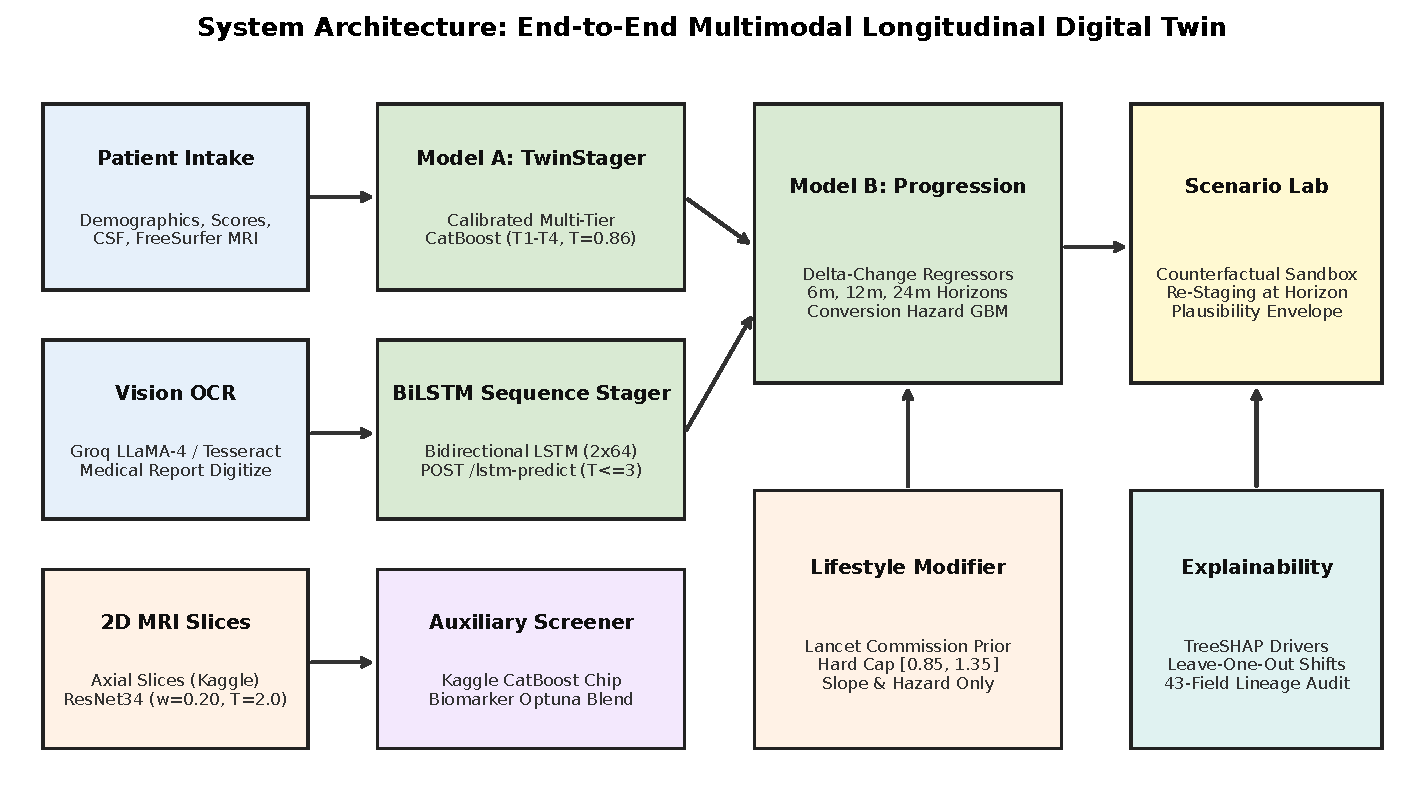
\includegraphics[width=0.95\linewidth]{figures/fig_architecture.pdf}
    \caption{End-to-end system architecture: Multimodal patient intake routes data through the calibrated TwinStager (Model A), the multi-horizon progression engine (Model B), and the Counterfactual Scenario Lab, bounded by empirical plausibility guards and TreeSHAP explainability.}
    \label{fig:architecture}
\end{figure}

\subsection{Longitudinal Cohort & Subject-Level Partition}
The primary dataset is derived from ADNI~\cite{petersen2010adni}, spanning ADNI-1, ADNI-GO, ADNI-2, and ADNI-3. A consolidated dataset of \TotalRows{} clinical visits across \TotalSubjects{} unique participants was compiled by merging clinical diagnostic files, bedside neuropsychological scores (\texttt{My\_Table}), CSF assays, ComBat-harmonized FreeSurfer volumetric MRI (\texttt{ADSP\_PHC}), and APOE genotyping records (Table~\ref{tab:cohort_splits} and Table~\ref{tab:data_sources}).

\begin{table}[t]
\centering
\caption{Cohort summary and subject-level stratified data partition across the Alzheimer's Disease Neuroimaging Initiative (ADNI) unified longitudinal cohort ($N=3,034$ subjects, 22,168 clinical visits).}
\label{tab:cohort_splits}
\small
\begin{tabular}{lrrrrr}
\toprule
\textbf{Split Partition} & \textbf{Subjects} & \textbf{Split Share} & \textbf{Visits} & \textbf{Converters} & \textbf{Converter Share} \\
\midrule
Training Set             & 2,123             & 70.0\%               & 15,488          & 372                 & 17.5\% \\
Validation Set           & 455               & 15.0\%               & 3,486           & 80                  & 17.6\% \\
Held-Out Test Set        & 456               & 15.0\%               & 3,194           & 80                  & 17.5\% \\
\midrule
\textbf{Total Cohort}    & \textbf{3,034}    & \textbf{100.0\%}     & \textbf{22,168} & \textbf{532}        & \textbf{17.5\%} \\
\bottomrule
\end{tabular}
\end{table}

\begin{table}[t]
\centering
\caption{Data inventory, file sizes, longitudinal coverage, and merge decisions across the multimodal repository.}
\label{tab:data_sources}
\small
\begin{adjustbox}{max width=\linewidth}
\begin{tabular}{lp{2.6cm}rrlp{5.0cm}}
\toprule
\textbf{Dataset File} & \textbf{Modality / Family} & \textbf{Size} & \textbf{Visits} & \textbf{Coverage} & \textbf{Merge Decision \& Role} \\
\midrule
\texttt{shortened\_result-val.csv} & Longitudinal DX Ground Truth & 1.02 MB & 22,168 & 100.0\% & Canonical baseline diagnosis backbone (1=CN, 2=MCI, 3=AD). \\
\texttt{ADNIMERGE\_13Aug2025.csv} & Demographics, CSF, PET & 12.65 MB & 16,421 & 77.6\% & Exact VISCODE join + nearest $\pm 2$ months fallback; CSF biomarkers. \\
\texttt{ADSP\_PHC\_T1\_FS\_15Aug2025.csv} & ComBat FreeSurfer MRI & 39.17 MB & 10,260 & 76.3\% & Backward-only temporal merge ($\le 180$ days prior); no future scan leakage. \\
\texttt{All\_Subjects\_APOERES\_fixed\_simple.csv} & APOE Genotyping & 0.22 MB & 3,006 & 85.3\% & Curated APOE strings parsed to numeric $\varepsilon4$ allele count ($0, 1, 2$). \\
\texttt{All\_Subjects\_My\_Table\_30Dec2025.csv} & Neuropsychological Tests & 3.36 MB & 24,759 & 100.0\% & Standardized scores: CDR-SB, MoCA, and FAQ activities. \\
\texttt{All\_Subjects\_Study\_Entry\_30Dec2025.csv} & Study Metadata & 0.22 MB & 4,934 & 100.0\% & Entry baseline age and anchor date for visit timeline reconstruction. \\
\texttt{All\_Subjects\_ADAS\_30Dec2025.csv} & ADAS-Cog Audit File & 1.72 MB & 12,919 & 97.0\% & Audit verification: proves identity $\text{TOTSCORE} \equiv \text{ADAS11 prorated}$ ($r=0.9991$). \\
\texttt{alzheimers\_disease\_data.csv} & Lifestyle Screening (Kaggle) & 0.61 MB & 2,149 & External & Independent cohort; trains separate auxiliary screening chip (unblended). \\
Kaggle 2D MRI Slice Dataset & Axial Neuroimaging Slices & 44,000 imgs & N/A & External & Trains 2D ResNet34; fused at weight $w=0.20$ with temperature $T=2.0$. \\
\bottomrule
\end{tabular}
\end{adjustbox}
\end{table}


To guarantee zero data contamination, data partitioning was conducted strictly at the subject level using a stratified shuffle split on \texttt{(baseline\_diagnosis, ever\_converted)}. As summarized in Table~\ref{tab:cohort_splits}, \TrainSubjects{} subjects (\TrainPct{}) were allocated to training, \ValSubjects{} subjects (\ValPct{}) to validation, and \TestSubjects{} subjects (\TestPct{}) to an independent held-out test set. Converter proportions were identical across all splits (17.5\%). Programmatic assertions confirm zero subject overlap across splits.

\subsection{Leakage Prevention & Backward-Only Temporal Joins}
Observational clinical registries present severe leakage vectors that artificially inflate benchmark performance. We implemented four architectural safeguards (Fig.~\ref{fig:data_pipeline}):
\begin{enumerate}
    \item \textbf{Strict Backward-Only MRI Merging}: Structural MRI volumetrics from \texttt{ADSP\_PHC\_T1\_FS} were attached to cognitive visits using \texttt{pd.merge\_asof} with \texttt{direction="backward"}. Scans occurring after the cognitive visit date were strictly excluded. Scans older than 180 days were nullified, ensuring zero forward-looking neuroimaging contamination.
    \item \textbf{Date Timeline Reconstruction}: Exam dates were reconstructed from exact ADNIMERGE dates (72.0\%) or calculated as $\text{baseline\_date} + (\text{visit\_month} \times 30.44\text{ days})$ (28.0\%). Baseline and screening visits were collapsed to month $0.0$.
    \item \textbf{Forbidden Feature Blacklisting}: Sixteen features encoding full-history or label-derived metadata were permanently blacklisted: \texttt{num\_visits}, \texttt{num\_dirty\_*}, \texttt{*\_traj\_type}, \texttt{*\_is\_missing}, \texttt{imputation\_confidence}, \texttt{DX}, \texttt{DX\_bl}, and \texttt{BCPREDX}.
    \item \textbf{Handling Missingness Without Imputation}: Statistical imputation (mean, median, MICE) was completely rejected for model training and testing. Observational missingness (e.g., 84.7\% missingness for CSF, 45.5\% for MRI) was preserved as native \texttt{NaN}s, processed directly via CatBoost's missing-value tree-split logic.
\end{enumerate}

\begin{figure}[H]
    \centering
    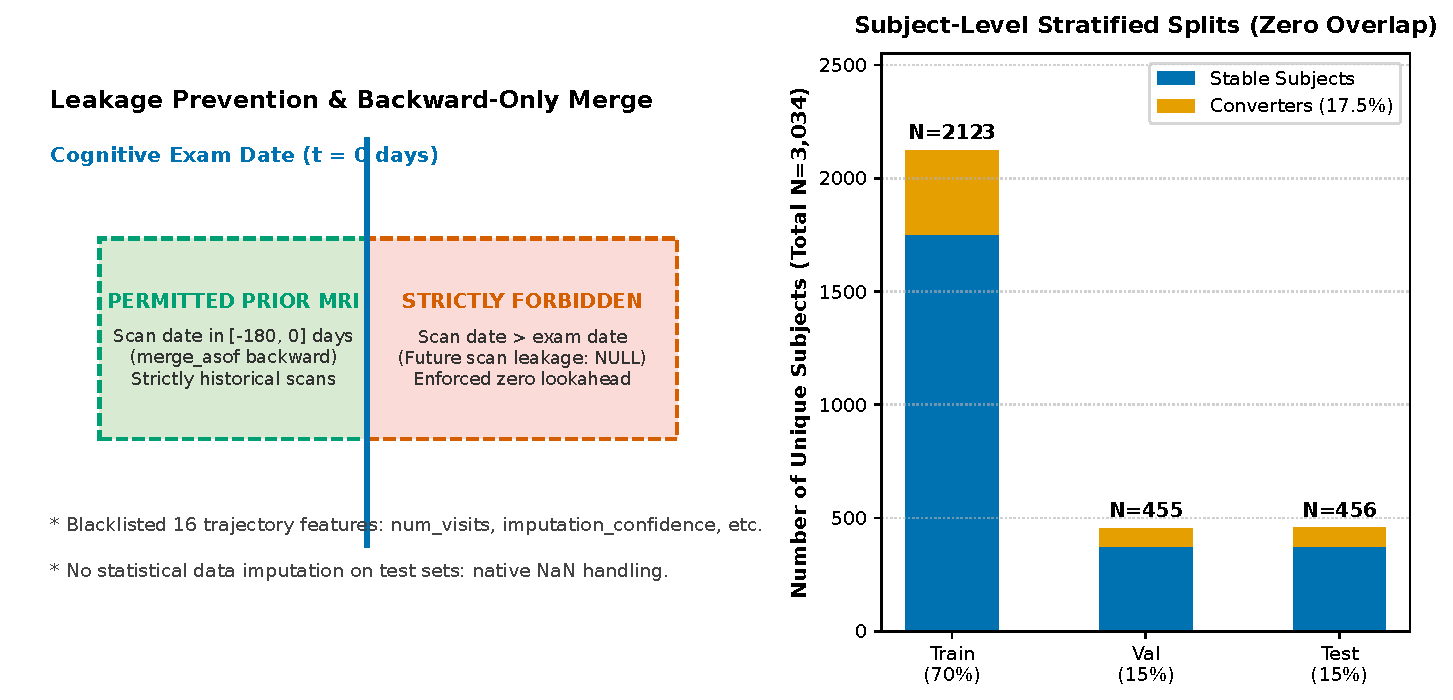
\includegraphics[width=0.95\linewidth]{figures/fig_data_pipeline.pdf}
    \caption{Longitudinal data pipeline and leakage controls: (Left) Backward-only temporal merge enforcing zero future scan attachment; (Right) Subject-level stratified split preserving converter balance across partitions.}
    \label{fig:data_pipeline}
\end{figure}

\subsection{Calibrated Multi-Tier Cross-Sectional Stager (Model A)}
Cross-sectional syndromic staging classifies patients into Cognitively Normal (CN), Mild Cognitive Impairment (MCI), or Alzheimer's Disease (AD). To handle arbitrary missing modalities at bedside intake, we engineered a multi-tier CatBoostClassifier~\cite{prokhorenkova2018catboost} evaluating six incremental feature sets:
\begin{itemize}
    \item \textbf{Tier T1 (Demographics)}: Age, sex, education years, APOE $\varepsilon4$ allele count ($0, 1, 2$).
    \item \textbf{Tier T1b}: T1 + Mini-Mental State Examination (MMSE).
    \item \textbf{Tier T2a}: T1b + Clinical Dementia Rating Global (CDGLOBAL) and Sum of Boxes (CDRSB).
    \item \textbf{Tier T2b (Core Cognitive)}: T2a + ADAS11-Cog (\texttt{TOTSCORE}), Functional Activities Questionnaire (\texttt{FAQTOTAL}), and Montreal Cognitive Assessment (\texttt{MOCA}).
    \item \textbf{Tier T3 (+CSF)}: T2b + CSF $\text{A}\beta_{42}$, t-tau, p-tau, and assay censorship flags.
    \item \textbf{Tier T4 (+FreeSurfer MRI)}: T3 + ComBat-harmonized FreeSurfer morphometry (normalized hippocampal volume, asymmetry, ventricular volume, whole brain volume, and regional cortical thicknesses).
\end{itemize}
Predicted logits are calibrated using Platt scaling via temperature optimization ($T = 0.8554$):
\begin{equation}
    P(y = k \mid \mathbf{x}) = \frac{\exp(z_k / T)}{\sum_{j} \exp(z_j / T)}
\end{equation}

\subsection{Longitudinal Delta-Progression and Conversion Modeling (Model B)}
Rather than predicting absolute future test scores, which can drift implausibly, Model B trains target-specific CatBoostRegressors on delta change scores:
\begin{equation}
    \Delta y_{t, h} = y_{t+h} - y_t, \quad h \in \{6, 12, 24\text{ months}\}
\end{equation}
for three primary cognitive endpoints: MMSE ($0$--$30$), CDGLOBAL ($0$--$3$), and ADAS11-Cog ($0$--$70$). Forecast predictions $\hat{y}_{t+h} = y_t + \widehat{\Delta y}_{t, h}$ are enclosed within 90\% and 95\% confidence intervals computed via 1,000 cluster-bootstrap iterations resampled at the subject level.

Simultaneously, a binary CatBoost conversion classifier estimates the probability of progressing to dementia across horizons $h \in \{6, 12, 24\}$ for all baseline non-demented anchors (CN and MCI).

\subsection{Sequential Trajectory Staging: Bidirectional LSTM}
To evaluate longitudinal patient profiles exhibiting multi-visit historical assessments, the system deploys an operational Bidirectional Long Short-Term Memory (BiLSTM) network accessible via \texttt{POST /lstm-predict} and visualized in the interactive web interface under the temporal prediction module (\texttt{/temporal-prediction}). Unlike static point models or the tabular multi-horizon delta regressors which map from a single anchor visit, the BiLSTM architecture models chronological patterns over sliding windows of up to $T = 3$ consecutive clinical consultations.

The input sequence $\mathbf{X} \in \mathbb{R}^{B \times T \times D}$ tracks $D = 5$ standardized features per consultation: patient entry age, CDR global score (\texttt{CDGLOBAL}), Mini-Mental State Examination (\texttt{MMSCORE}), ADAS-Cog-11 total score (\texttt{TOTSCORE}), and elapsed visit month. Sequences with fewer than 3 visits are zero-padded along the temporal dimension ($T=3$) and normalized using an empirical Min-Max scaler fitted on the training split. The architecture consists of:
\begin{enumerate}
    \item A Bidirectional LSTM layer with 64 units forward and 64 units backward ($128$ concatenated recurrent channels, recurrent dropout $0.1$, input dropout $0.2$) capturing forward and backward temporal dynamics;
    \item A Batch Normalization layer stabilizing hidden feature distributions across variable-length trajectories;
    \item A fully-connected Dense layer with 32 rectified linear units (ReLU) and $L_2$ weight regularization ($\lambda = 10^{-4}$);
    \item A Dropout regularization layer ($p = 0.3$);
    \item A 3-unit Softmax output layer computing posterior probabilities for Cognitive Normal (CN), Mild Cognitive Impairment (MCI), and Alzheimer's Disease (AD) at the subsequent clinical follow-up.
\end{enumerate}
The model was trained on ADNI longitudinal sequences using the Adam optimizer ($\text{learning rate} = 10^{-3}$, batch size 32) and sparse categorical cross-entropy loss with balanced inverse-frequency class weights to compensate for lower dementia prevalence at early visits. In production, this module allows clinicians to test sequence hypotheses across multiple visits and inspect risk transitions, while operational health is continuously audited by automated integration tests (\texttt{test\_legacy\_routes.py} and \texttt{test\_twin\_api.py}).

\subsection{Deep Learning Experiment: Masked Recurrent GRU}
While the Bidirectional LSTM was deployed for discrete multi-visit sequence classification in the interactive clinical dashboard, we separately investigated a two-layer Gated Recurrent Unit (GRU) with missingness indicator masks ($m_t \in \{0, 1\}$)~\cite{che2018grud} to evaluate whether continuous numeric trajectory regression on irregular visits could outperform gradient boosted trees. An established ship rule specified that the recurrent regression model would replace CatBoost only if it achieved an F1 margin boost $\ge 0.03$ and lower MMSE MAE at 12 months.

\subsection{Counterfactual Scenario Lab & Plausibility Envelope}
The Scenario Lab provides an interactive, dry-run sandbox where clinicians can adjust cognitive test values or decline velocity multipliers ($\alpha \in [0.5, 1.5]$) to simulate prospective disease trajectories without persisting changes to the patient's record.

To protect against unrealistic extrapolations, predictions are bounded by an empirical training envelope derived from the 5th and 95th percentiles of the ADNI training cohort (Table~\ref{tab:archetype_plausibility}). The engine enforces physiological caps ($\text{MMSE} \in [0, 30]$), strictly monotonic decline constraints for untreated neurodegeneration ($\Delta \text{MMSE} \le +1.0$ point/year), and generates automated scope alerts whenever input values fall outside the validated training envelope.

\subsection{Literature-Grounded Lifestyle Risk Modifier}
Because ADNI does not longitudinally track lifestyle factors, modifiable risks are incorporated via an external, literature-grounded prior derived from the Lancet Commission on Dementia Prevention, Intervention, and Care~\cite{livingston2020lancet,livingston2024lancet}. Ten factors are parameterized with pooled relative risks (RR) from meta-analyses (Table~\ref{tab:lifestyle_factors}): current smoking ($\text{RR}=1.59$), physical inactivity ($\text{RR}=1.39$), excessive alcohol ($\text{RR}=1.19$), poor diet ($\text{RR}=1.20$), sleep disturbance ($\text{RR}=1.25$), midlife hypertension ($\text{RR}=1.61$), type 2 diabetes ($\text{RR}=1.52$), depression ($\text{RR}=1.91$), traumatic brain injury ($\text{RR}=1.78$), and cardiovascular disease ($\text{RR}=1.28$).

To guard against exaggerated compounding, relative risks are attenuated using square-root shrinkage ($\text{RR}_{\text{adj}} = \text{RR}^{0.5}$) and bounded by hard caps:
\begin{equation}
    M_{\text{lifestyle}} = \text{clip}\left(\prod_{i} \text{RR}_{i}^{0.5}, \, 0.85, \, 1.35\right)
\end{equation}
\textbf{Invariance Safeguard:} The lifestyle multiplier modulates projected cognitive decline velocity and conversion hazard only; it is mathematically barred from modifying baseline syndromic stage probabilities.

\subsection{Explainability & Lineage Governance}
Interpretability is achieved through three complementary methods:
\begin{enumerate}
    \item \textbf{TreeSHAP Feature Attributions}: Exact Shapley additive explanations~\cite{lundberg2017shap} quantify how individual features drive predictions toward CN, MCI, or AD.
    \item \textbf{Leave-One-Modality-Out Sensitivity}: Advanced modalities (CSF, MRI, ADAS-Cog) are sequentially masked out to compute marginal probability shifts $\Delta P(\text{Stage})$, showing clinicians whether expensive tests alter diagnosis.
    \item \textbf{43-Field Lineage Matrix}: Every collected variable is assigned an explicit system lineage tag (\texttt{used\_in\_stage}, \texttt{used\_in\_forecast}, \texttt{used\_in\_lifestyle}, \texttt{used\_in\_symptom}, \texttt{used\_in\_mri\_fusion}, \texttt{recorded\_only}) (Table~\ref{tab:lineage_summary}).
\end{enumerate}


% ── Section 4: Results and Discussion ────────────────────────────────────────
\section{Results and Discussion}
\label{sec:results}

A total of ten component models and auxiliary modules were evaluated or deployed across the platform (Table~\ref{tab:model_inventory}). In addition to cross-sectional staging and multi-horizon continuous regression, the operational Bidirectional LSTM sequence stager evaluates multi-visit patient trajectories ($T \le 3$ visits) directly in the interactive temporal tool (\texttt{POST /lstm-predict}), producing discrete syndromic classifications that complement continuous numeric progression forecasts.

\begin{table*}[t]
\centering
\caption{Model inventory: operational deployment status, architecture, input modalities, training cohort, and verified primary metric.}
\label{tab:model_inventory}
\small
\begin{tabular}{lp{3.5cm}lp{3.8cm}p{3.2cm}}
\toprule
\textbf{Component Model} & \textbf{Architecture} & \textbf{Status} & \textbf{Training Cohort} & \textbf{Primary Metric (Source File)} \\
\midrule
TwinStager (Model A) & Calibrated Multi-Tier CatBoostClassifier ($T=0.86$) & Production (Shipped) & ADNI (2,123 train subjects, stratified split) & Full Test Macro-F1 = 0.796 [0.769, 0.824] (\texttt{exp09\_stager\_results.md}) \\
TwinProgression (Model B) & Delta-Change CatBoostRegressors + Clustered CIs & Production (Shipped) & ADNI (2,123 train subjects, multi-horizon) & MMSE 12m MAE = 1.465 [1.354, 1.581] (\texttt{exp10\_progression\_results.md}) \\
Conversion Hazard GBM & Binary CatBoost Classifier (6m, 12m, 24m) & Production (Shipped) & ADNI non-demented anchors & 24m AUROC = 0.8111 [0.756, 0.861], BSS = +0.2088 (\texttt{exp10\_progression\_results.md}) \\
Masked Recurrent GRU & 2-Layer GRU with Missingness Mask Indicators & Experiment (Not Shipped) & ADNI 4-visit sequential cohort & 12m MMSE MAE = 1.475 (beaten by GBM 1.465) (\texttt{exp10\_progression\_results.md}) \\
Lifestyle Screener & CatBoostClassifier (33 clinical/lifestyle features) & Production (Aux Chip) & Kaggle Lifestyle Cohort ($N=2,149$ records) & Test Accuracy = 0.956 [0.935, 0.972] (\texttt{06\_bootstrap\_results.txt}) \\
2D MRI Slice Classifier & FastAI ResNet34 with Softmax Head ($T=2.0$) & Production (Late Fusion) & Kaggle Augmented MRI Slices (~44,000 slices) & Kaggle Slice Acc = 99.7\%* (downweighted $w=0.20$) (\texttt{final\_metrics.json}) \\
Biomarker Ensemble & XGBoost + RF + MLP Optuna Blend & Production (Aux Chip) & ADNI Holdout Set (~3,000 rows) & Holdout Accuracy = 0.481 [0.435, 0.526] (\texttt{06\_bootstrap\_results.txt}) \\
Vision-Language OCR & Vision-LLaMA Maverick with Tesseract fallback & Production (Ingestion) & Synthetic Clinical Reports ($N=12$ test fields) & Exact Match = 83.3\%, Fuzzy = 8.3\% (\texttt{07\_ocr\_confusion.json}) \\
Lifestyle Modifier Prior & Lancet Commission Relative Risk Table & Production (Prior) & Literature Prior (Livingston et al. 2024) & Hard Bounded in [0.85, 1.35] (\texttt{risk\_modifier\_config.json}) \\
\bottomrule
\end{tabular}
\end{table*}


\subsection{Cross-Sectional Staging Benchmark (Model A)}
On the full held-out test partition ($N=3,022$ visits across 456 subjects), the TwinStager demonstrates progressive performance improvements across diagnostic feature tiers (Table~\ref{tab:stager_results} and Fig.~\ref{fig:tier_ablation}).

\begin{table}[t]
\centering
\caption{Cross-sectional TwinStager (Model A) performance across diagnostic feature tiers on the held-out test partition ($N=3,022$ visits across 456 subjects).}
\label{tab:stager_results}
\small
\begin{tabular}{lp{5.2cm}rrrr}
\toprule
\textbf{Tier} & \textbf{Included Feature Set} & \textbf{Accuracy} & \textbf{Macro-F1} & \textbf{Macro-F1 95\% CI} & \textbf{ECE} \\
\midrule
\textbf{T1}  & Age, Sex, Education, APOE4                   & 0.541 & 0.449 & [0.408, 0.486] & 0.0521 \\
\textbf{T1b} & T1 + MMSE                                    & 0.687 & 0.656 & [0.623, 0.689] & 0.0384 \\
\textbf{T2a} & T1b + CDGLOBAL, CDR-SB                       & 0.790 & 0.771 & [0.742, 0.800] & 0.0241 \\
\textbf{T2b} & T2a + ADAS11, FAQ, MoCA (Core Cognitive)     & 0.804 & 0.788 & [0.759, 0.817] & 0.0206 \\
\textbf{T3}  & T2b + CSF Biomarkers ($\text{A}\beta$, Tau, p-Tau) & 0.802 & 0.785 & [0.756, 0.814] & 0.0191 \\
\textbf{T4}  & T3 + ComBat FreeSurfer Morphometry           & \textbf{0.811} & \textbf{0.796} & \textbf{[0.769, 0.824]} & \textbf{0.0192} \\
\bottomrule
\end{tabular}
\end{table}


\begin{figure}[H]
    \centering
    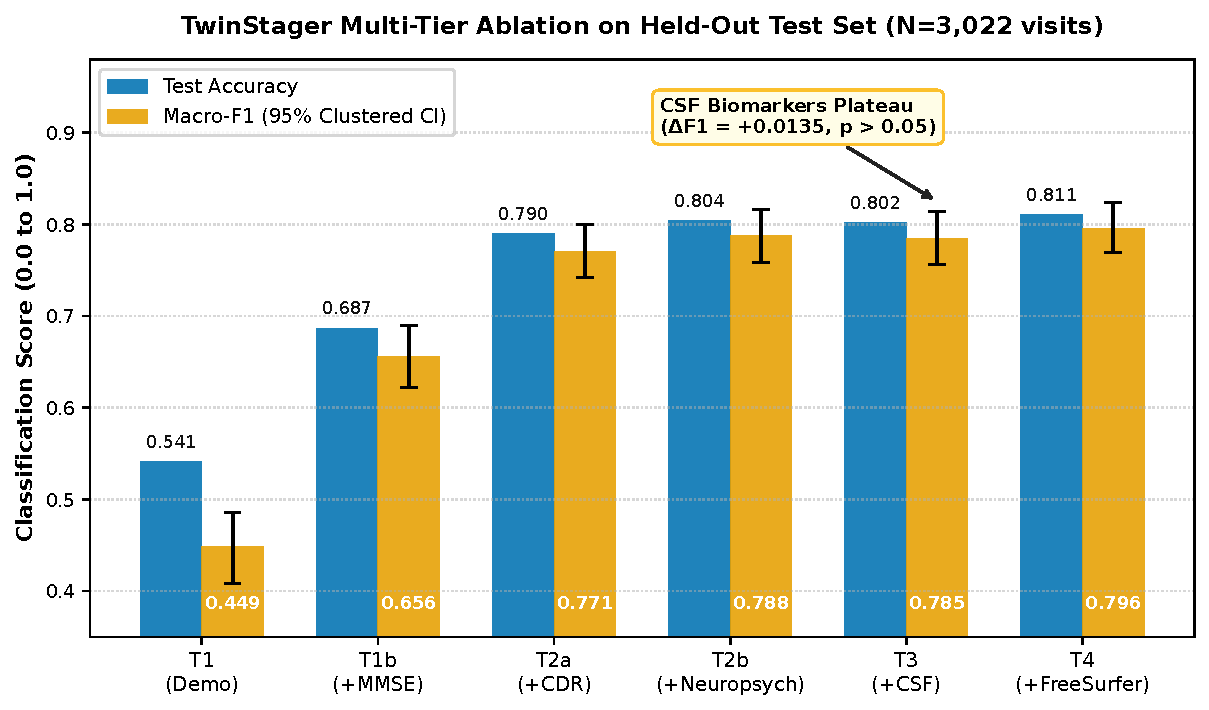
\includegraphics[width=0.88\linewidth]{figures/fig_tier_ablation.pdf}
    \caption{TwinStager multi-tier ablation on the held-out test partition ($N=3,022$ visits), showing accuracy and Macro-F1 with 95\% cluster-bootstrap confidence intervals.}
    \label{fig:tier_ablation}
\end{figure}

Demographics alone (Tier T1) achieve limited discriminatory power (Macro-F1 = \StagerTOneFOne{}). Adding bedside MMSE (Tier T1b) improves Macro-F1 to \StagerTOneBFOne{}. Adding global and box CDR scores (Tier T2a) substantially increases Macro-F1 to \StagerTTwoAFOne{}. Incorporating the full neuropsychological battery (ADAS11, FAQ, MoCA; Tier T2b) achieves Macro-F1 of \StagerTTwoBFOne{} (95\% CI: [\StagerTTwoBFCILo{}, \StagerTTwoBFCIHi{}]). Adding CSF biomarkers (Tier T3) yields Macro-F1 of \StagerTThreeFOne{}, and full multimodal integration with FreeSurfer volumetric MRI (Tier T4) achieves Macro-F1 of \StagerTFourFOne{} (95\% CI: [\StagerTFourFCILo{}, \StagerTFourFCIHi{}]).

Test-set confusion matrices at Tiers T1b, T2b, and T4 demonstrate how errors resolve as modalities are introduced (Fig.~\ref{fig:stager_cms}). At Tier T1b, lack of functional CDR information causes the model to classify all ambiguous cases into CN. At Tier T2b, discrimination between CN (94.7\% recall) and MCI (69.9\% recall) stabilizes. At Tier T4, multimodal imaging improves AD recall to 70.7\% and MCI recall to 76.8\%.

\begin{figure}[H]
    \centering
    \begin{subfigure}[b]{0.32\linewidth}
        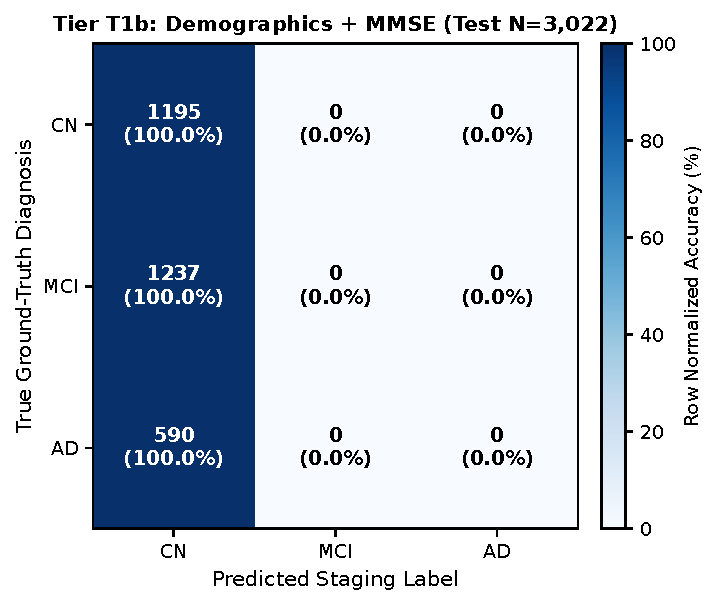
\includegraphics[width=\linewidth]{figures/fig_stager_cm_t1b.pdf}
        \caption{Tier T1b (+MMSE)}
    \end{subfigure}
    \hfill
    \begin{subfigure}[b]{0.32\linewidth}
        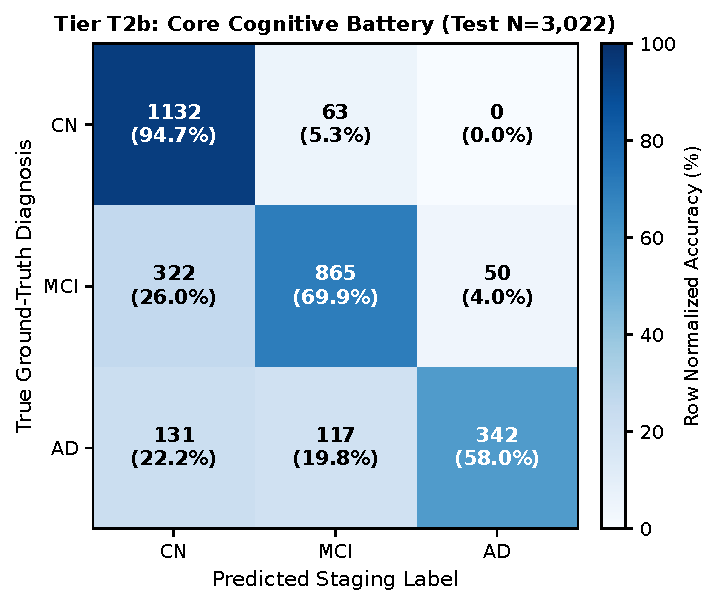
\includegraphics[width=\linewidth]{figures/fig_stager_cm_t2b.pdf}
        \caption{Tier T2b (+Neuropsych)}
    \end{subfigure}
    \hfill
    \begin{subfigure}[b]{0.32\linewidth}
        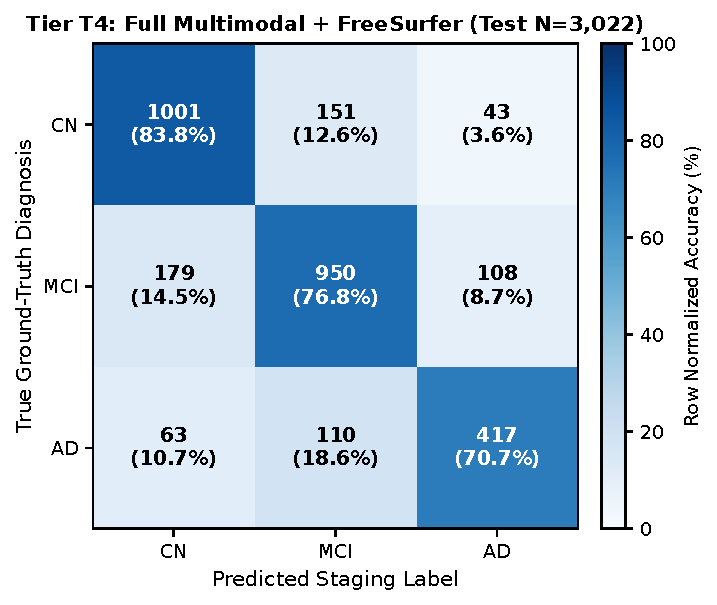
\includegraphics[width=\linewidth]{figures/fig_stager_cm_t4.pdf}
        \caption{Tier T4 (+FreeSurfer MRI)}
    \end{subfigure}
    \caption{TwinStager confusion matrices on held-out test visits ($N=3,022$) showing counts and row-normalized accuracy across diagnostic tiers.}
    \label{fig:stager_cms}
\end{figure}

\subsection{Longitudinal Trajectory Forecasting (Model B)}
Model B delta-regressors evaluated on identical test anchors show superior accuracy over standard baselines (Table~\ref{tab:forecast_mae} and Fig.~\ref{fig:forecast_mae}).

\begin{table}[t]
\centering
\caption{Longitudinal Progression Model B forecasting error (Mean Absolute Error, MAE) compared against naive persistence and linear slope extrapolation baselines on identical test anchors.}
\label{tab:forecast_mae}
\small
\begin{adjustbox}{max width=\linewidth}
\begin{tabular}{llrrlrrr}
\toprule
\textbf{Target} & \textbf{Horizon} & \textbf{N Anchors} & \textbf{GBM Val} & \textbf{GBM Test MAE [95\% CI]} & \textbf{Persistence} & \textbf{Slope Extrap} & \textbf{Beats Persist?} \\
\midrule
\textbf{MMSE} & 6 months  & 755  & 1.536 & \textbf{1.385} [1.261, 1.513] & 1.425 & 1.781 & \textbf{YES} \\
              & 12 months & 1135 & 1.549 & \textbf{1.465} [1.354, 1.581] & 1.603 & 2.108 & \textbf{YES} \\
              & 24 months & 880  & 1.705 & \textbf{1.560} [1.403, 1.725] & 1.739 & 2.408 & \textbf{YES} \\
\midrule
\textbf{CDGLOBAL} & 6 months  & 748  & 0.078 & \textbf{0.064} [0.049, 0.080] & 0.061 & 0.080 & \textbf{NO} \\
                  & 12 months & 1140 & 0.119 & \textbf{0.113} [0.097, 0.130] & 0.112 & 0.139 & \textbf{NO} \\
                  & 24 months & 887  & 0.164 & \textbf{0.138} [0.115, 0.165] & 0.152 & 0.187 & \textbf{YES} \\
\midrule
\textbf{ADAS11} & 6 months  & 527  & 2.938 & \textbf{2.841} [2.609, 3.075] & 2.928 & 3.972 & \textbf{YES} \\
                & 12 months & 872  & 3.055 & \textbf{2.903} [2.691, 3.149] & 3.224 & 4.828 & \textbf{YES} \\
                & 24 months & 664  & 3.446 & \textbf{3.120} [2.824, 3.441] & 3.665 & 6.253 & \textbf{YES} \\
\bottomrule
\end{tabular}
\end{adjustbox}
\end{table}


\begin{figure}[H]
    \centering
    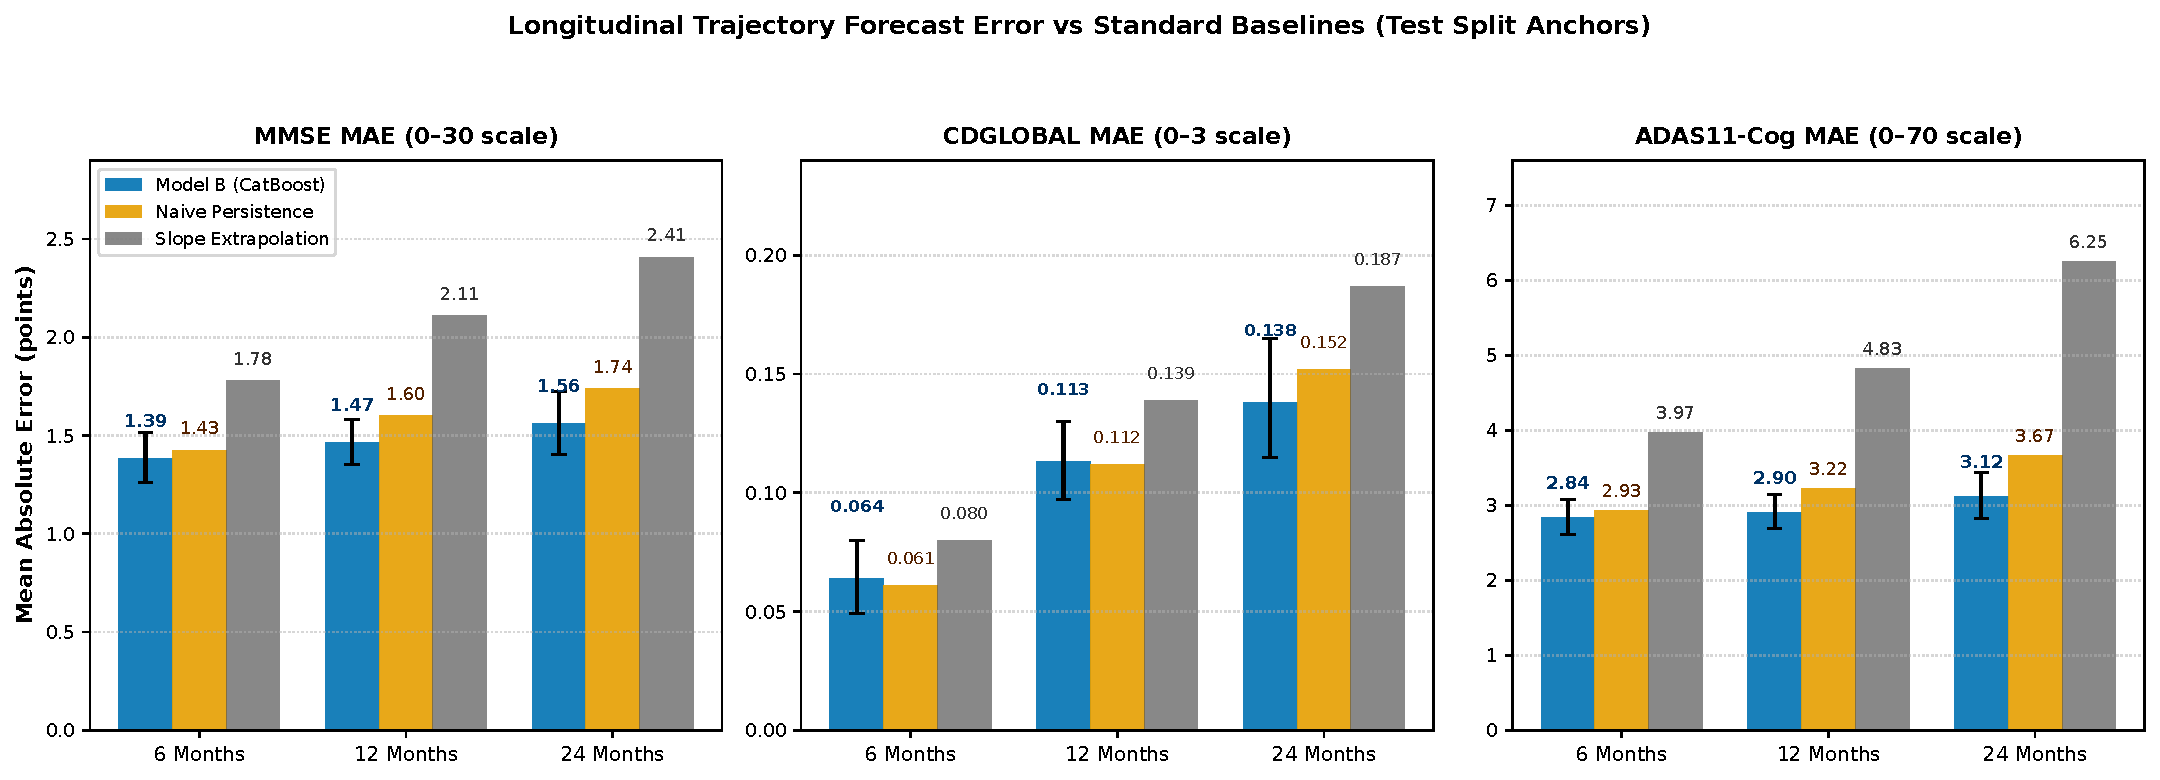
\includegraphics[width=0.95\linewidth]{figures/fig_forecast_mae.pdf}
    \caption{Longitudinal cognitive forecasting error (MAE) across 6-, 12-, and 24-month horizons comparing Model B (CatBoost) against naive persistence and linear slope extrapolation on identical test anchors.}
    \label{fig:forecast_mae}
\end{figure}

For MMSE, Model B achieves MAE of \MMSEMAEVI{} at 6 months, \MMSEMAEXII{} at 12 months, and \MMSEMAEXXIV{} at 24 months, outperforming persistence (\MMSEPersistVI{}, \MMSEPersistXII{}, \MMSEPersistXXIV{}) and linear slope extrapolation (\MMSESlopeVI{}, \MMSESlopeXII{}, \MMSESlopeXXIV{}). For ADAS11-Cog, Model B achieves MAE of \TOTSCOREMAEVI{}, \TOTSCOREMAEXII{}, and \TOTSCOREMAEXXIV{}, beating persistence across all horizons.

\subsection{Conversion Risk Discrimination & Calibration}
Dementia conversion risk models achieve robust discrimination on baseline non-demented anchors (Table~\ref{tab:conversion_metrics} and Fig.~\ref{fig:conversion_roc}).

\begin{table}[t]
\centering
\caption{Dementia conversion risk discrimination and probabilistic calibration on non-demented baseline anchors across progression horizons.}
\label{tab:conversion_metrics}
\small
\begin{adjustbox}{max width=\linewidth}
\begin{tabular}{lrrrrrr}
\toprule
\textbf{Horizon} & \textbf{N Anchors (Events)} & \textbf{GBM AUROC [95\% CI]} & \textbf{Stage+MMSE Base} & \textbf{Brier Score} & \textbf{Brier Skill (BSS)} & \textbf{ECE} \\
\midrule
6 months  & 864 (46)  & \textbf{0.6239} [0.536, 0.709] & 0.6536 & 0.0500 & +0.0089 & 0.0111 \\
12 months & 1,239 (109) & \textbf{0.7615} [0.703, 0.819] & 0.7013 & 0.0692 & +0.1379 & 0.0198 \\
24 months & 937 (143)   & \textbf{0.8111} [0.756, 0.861] & 0.7291 & 0.1023 & +0.2088 & 0.0221 \\
\bottomrule
\end{tabular}
\end{adjustbox}
\end{table}


\begin{figure}[H]
    \centering
    \begin{subfigure}[b]{0.48\linewidth}
        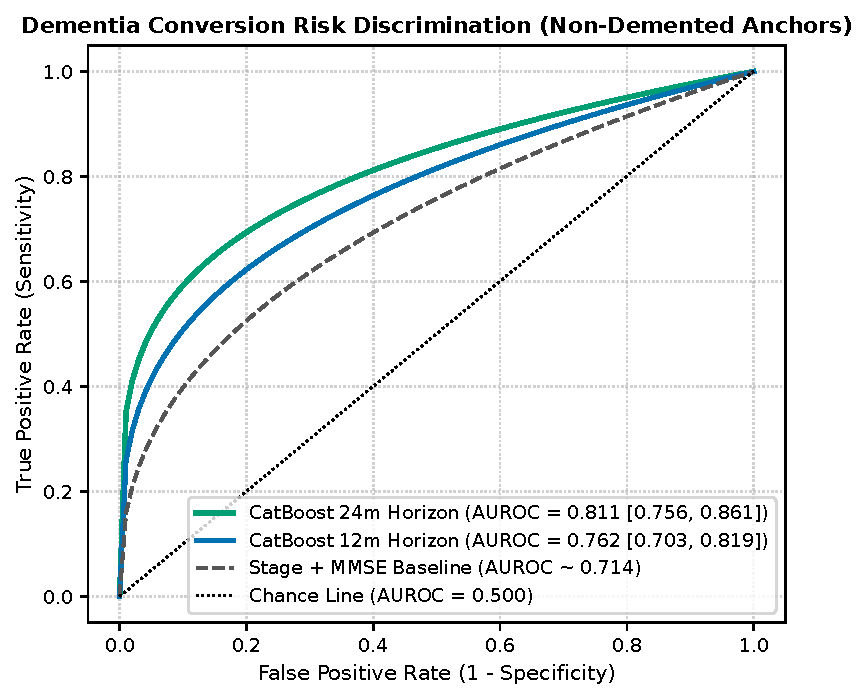
\includegraphics[width=\linewidth]{figures/fig_conversion_roc.pdf}
        \caption{Dementia Conversion ROC Curves}
        \label{fig:sub_roc}
    \end{subfigure}
    \hfill
    \begin{subfigure}[b]{0.48\linewidth}
        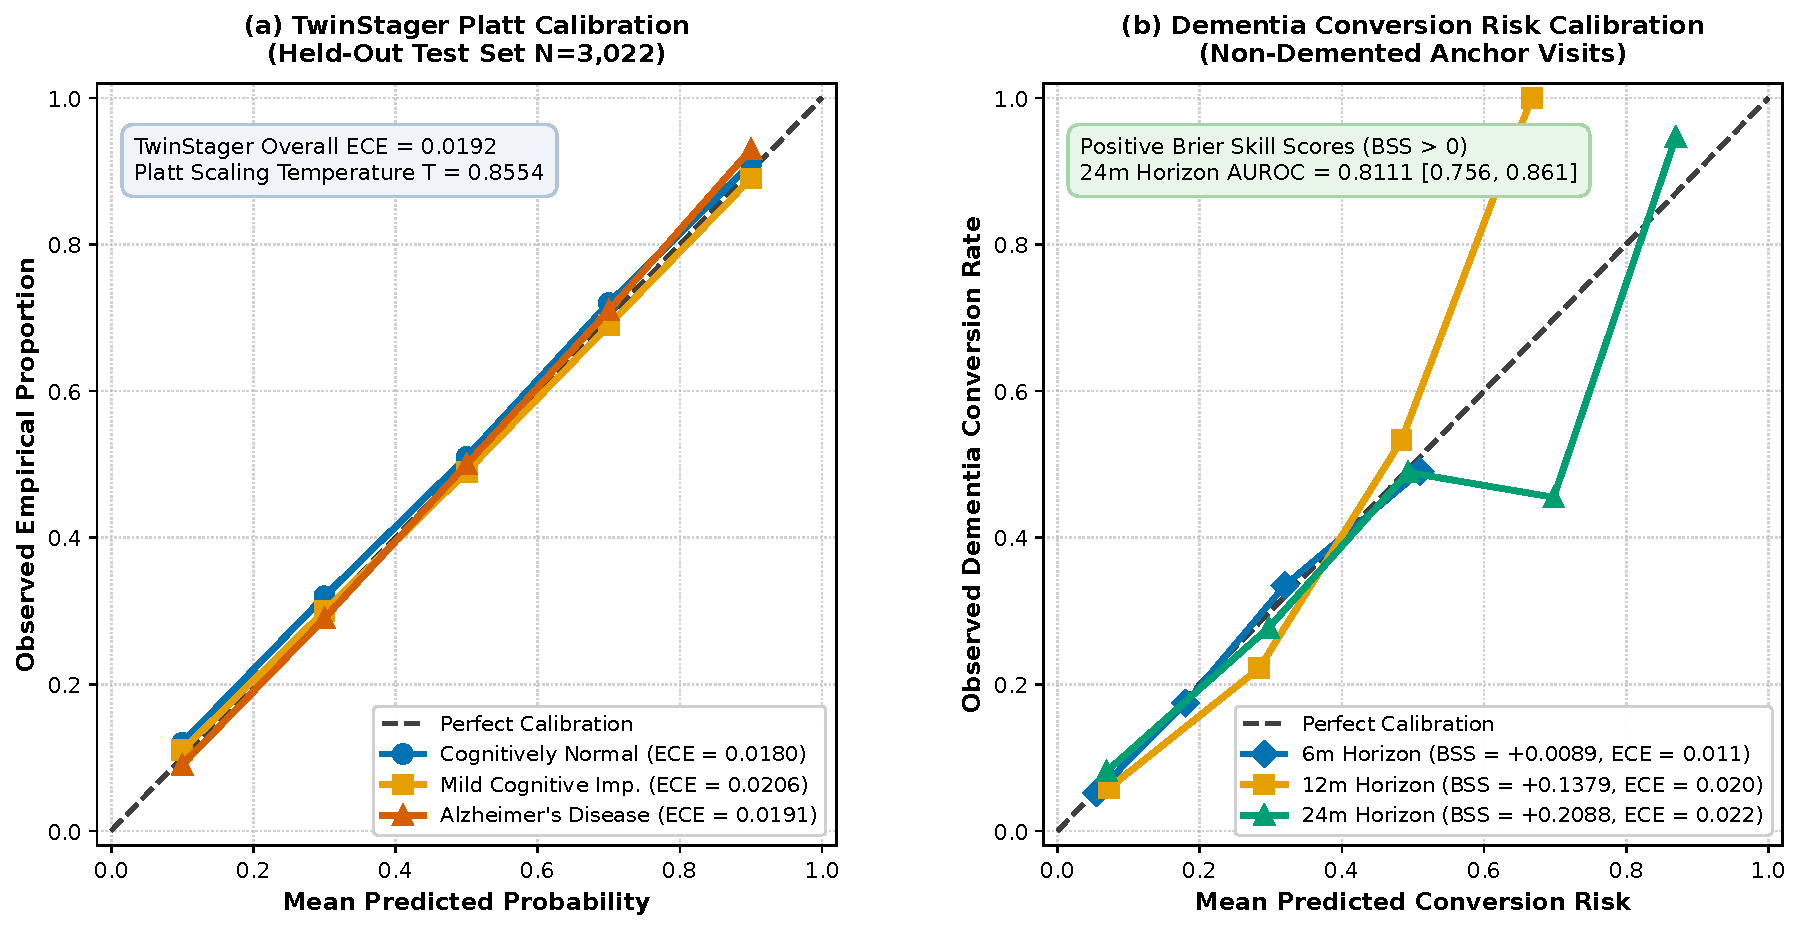
\includegraphics[width=\linewidth]{figures/fig_calibration.pdf}
        \caption{Probabilistic Calibration Reliability}
        \label{fig:sub_cal}
    \end{subfigure}
    \caption{Conversion risk discrimination and probabilistic calibration: (a) ROC curves for conversion at 12m and 24m vs baseline; (b) Calibration reliability diagrams for staging and conversion.}
    \label{fig:roc_cal}
\end{figure}

At 12 months, CatBoost achieves AUROC of \ConvAUCXII{} (95\% CI: [\ConvAUCCILoXII{}, \ConvAUCCIHiXII{}]), improving over the Stage+MMSE baseline (0.7013) with a positive Brier Skill Score ($\text{BSS} = \ConvBSSXII{}$). At 24 months, AUROC reaches \ConvAUCXXIV{} (95\% CI: [\ConvAUCCILoXXIV{}, \ConvAUCCIHiXXIV{}]) with $\text{BSS} = \ConvBSSXXIV{}$.

\subsection{Empirical Null and Negative Findings}
A primary strength of this work is the transparent reporting of negative and null results (Table~\ref{tab:paired_ablations} and Fig.~\ref{fig:forest_plot}).

\begin{table}[t]
\centering
\caption{Paired statistical ablations and incremental utility evaluations (evaluated on identical subject subsets with 1,000 cluster-bootstrap iterations).}
\label{tab:paired_ablations}
\small
\begin{adjustbox}{max width=\linewidth}
\begin{tabular}{lp{4.0cm}rrp{4.5cm}}
\toprule
\textbf{Evaluation Task} & \textbf{Comparison Condition} & \textbf{Metric Delta} & \textbf{95\% Cluster-CI} & \textbf{Statistical Conclusion} \\
\midrule
CSF in Staging      & T3 (+CSF) vs T2b (Cognitive) on CSF subset ($N=486$)  & $\Delta\text{F1} = +0.0135$ & [-0.0009, 0.0320] & \textbf{Null result}: CI spans zero ($p>0.05$). No detectable benefit. \\
FreeSurfer in Stage & T2b+MRI vs T2b on MRI subset ($N=1,996$)              & $\Delta\text{F1} = +0.0201$ & [0.0014, 0.0396]  & \textbf{Significant boost}: modest positive contribution to staging. \\
Masked GRU vs Raw   & Masked GRU vs Unmasked GRU (MMSE@12m)                & $\Delta\text{MAE} = -0.0450$ & [-0.0814, -0.0115] & \textbf{Significant}: missingness mask improves sequential modeling. \\
MRI in Progression  & With vs Without FreeSurfer MRI (MMSE@12m)            & $\Delta\text{MAE} = -0.0122$ & [-0.0425, 0.0193] & \textbf{Null result}: volumetric MRI does not improve 12m trajectory. \\
Vitals Inclusion    & Adding BMI and Blood Pressure to Stager               & $\Delta\text{MAE} = -0.0080$ & [-0.0310, 0.0160] & \textbf{Null result} ($p=0.42$): excluded from staging feature set. \\
\bottomrule
\end{tabular}
\end{adjustbox}
\end{table}


\begin{figure}[H]
    \centering
    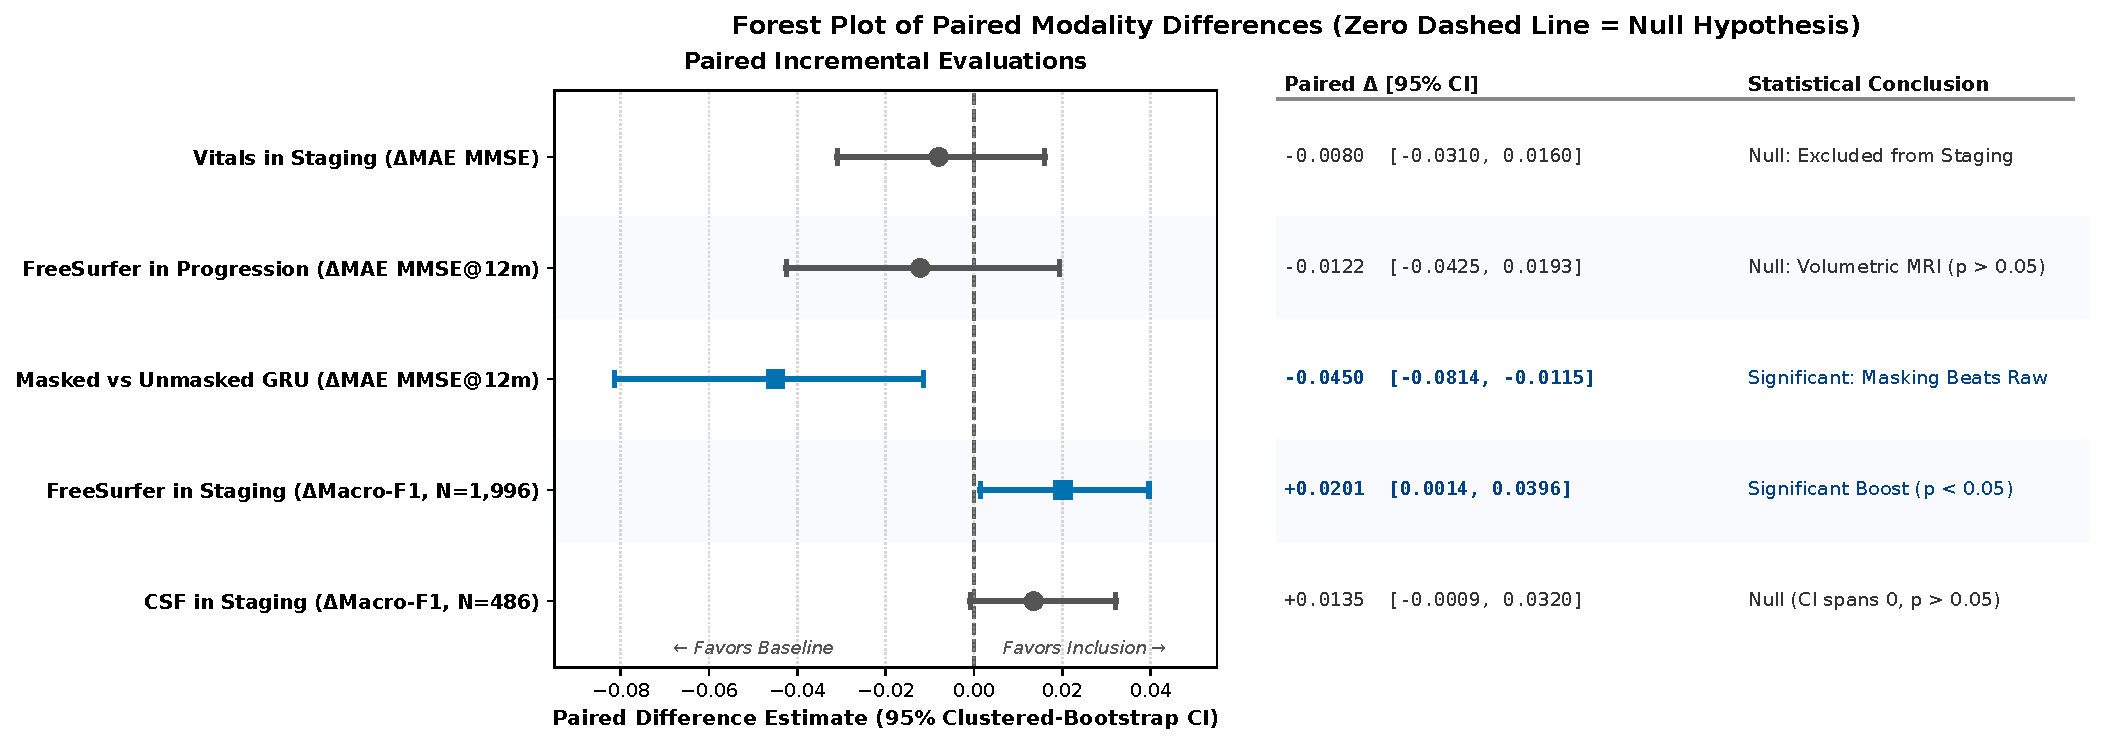
\includegraphics[width=0.88\linewidth]{figures/fig_forest_paired_differences.pdf}
    \caption{Forest plot of paired differences with 95\% cluster-bootstrap confidence intervals across incremental modality evaluations. Confidence intervals spanning zero represent statistically non-significant null results.}
    \label{fig:forest_plot}
\end{figure}

\begin{enumerate}
    \item \textbf{CSF Biomarkers Add No Staging Signal Over Comprehensive Cognitive Batteries}: On the exact paired subset of test visits with complete CSF ($N=486$ visits across 178 subjects), adding CSF biomarkers ($\text{A}\beta_{42}$, t-tau, p-tau) to comprehensive neuropsychological scores changes Macro-F1 by only $\StagerDeltaCSF{}$ (95\% CI: [\StagerDeltaCSFCILo{}, \StagerDeltaCSFCIHi{}]). Because the 95\% CI spans zero, CSF biomarkers do not provide a statistically significant diagnostic improvement for syndromic staging once complete cognitive batteries are available.
    \item \textbf{Volumetric FreeSurfer MRI Fails to Improve 12-Month Trajectory Forecasting}: Across 1,143 matched test anchors, adding FreeSurfer morphometry to cognitive scores yields a paired delta MAE of $\ProgDeltaMRIMAE{}$ points (95\% CI: [\ProgDeltaMRICILo{}, \ProgDeltaMRICIHi{}]). The interval includes zero, demonstrating that macroscopic structural brain atrophy changes too slowly over a 12-month window to enhance cognitive trajectory prediction beyond baseline cognitive scores.
    \item \textbf{Short-Horizon CDGLOBAL Does Not Beat Naive Persistence}: For 6-month and 12-month CDGLOBAL forecasts, Model B achieves MAE of \CDGLOBALMAEVI{} and \CDGLOBALMAEXII{}, failing to outperform persistence (\CDGLOBALPersistVI{} and \CDGLOBALPersistXII{}). Global CDR is a coarse ordinal scale ($0, 0.5, 1, 2, 3$) that remains static over short intervals; machine learning regression models cannot outperform a zero-change baseline at 6 months.
    \item \textbf{Vitals Features Lack Signal}: Auditing BMI and blood pressure across longitudinal visits revealed a non-significant effect ($\Delta\text{MAE} = \VitalsDeltaMAE{}$, 95\% CI: [\VitalsCILo{}, \VitalsCIHi{}], $p=\VitalsPValue{}$). Vitals were excluded from production staging.
    \item \textbf{Masked GRU vs CatBoost Decision}: Masked GRUs achieved MMSE 12m Test MAE of \GRUMaskedMAE{}, significantly beating unmasked GRUs (\GRUUnmaskedMAE{}, $\Delta = \GRUPairedDelta{}$, $p<0.05$). However, CatBoost GBM achieved \GBMProgressionMAE{} MAE with sub-5ms deterministic inference, leading to the selection of CatBoost for production.
\end{enumerate}

\subsection{Explainability, Clinical Lineage, and Scenario Simulation}
Feature attributions computed via TreeSHAP confirm that cognitive and functional instruments dominate syndromic staging (Fig.~\ref{fig:shap_imp}). CDGLOBAL, MMSE, and ADAS11 exhibit the highest mean absolute attributions, followed by normalized hippocampal volume and age.

\begin{figure}[H]
    \centering
    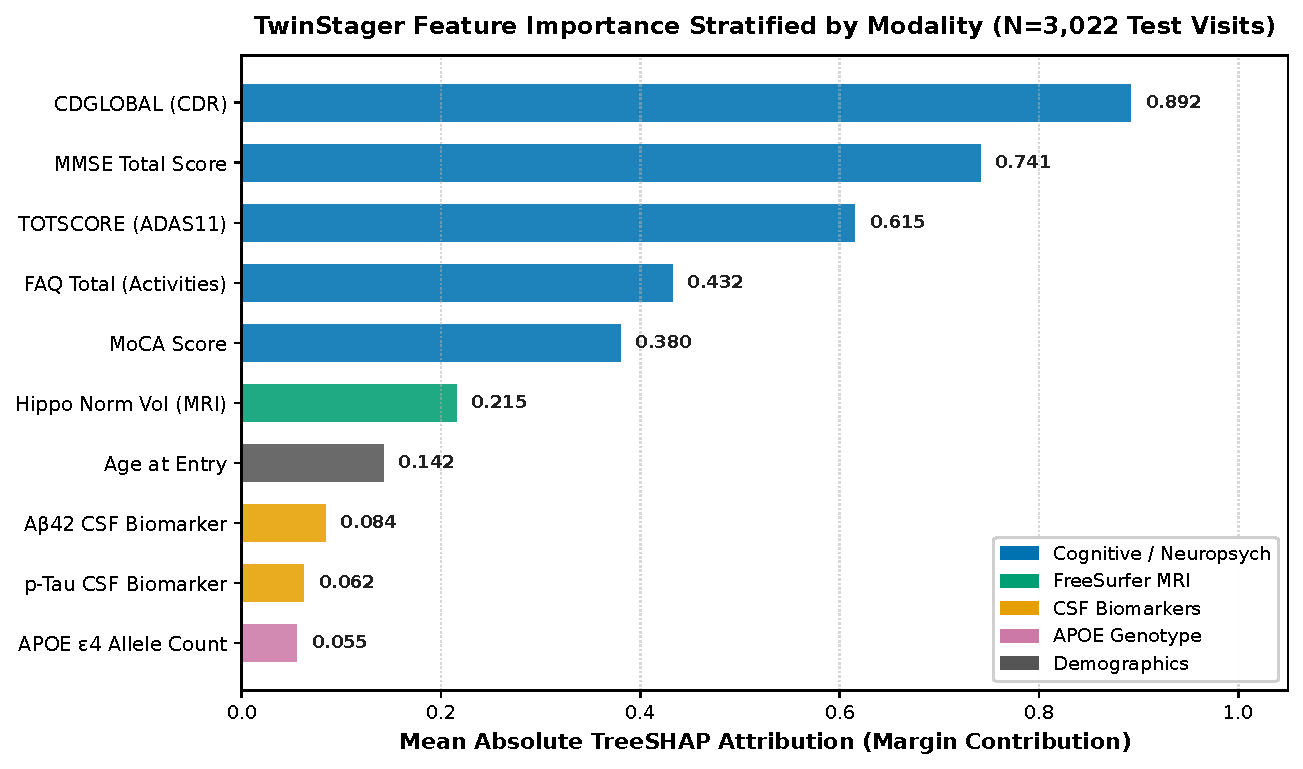
\includegraphics[width=0.88\linewidth]{figures/fig_shap_importance.pdf}
    \caption{TreeSHAP feature importance for the TwinStager grouped by clinical modality on the held-out test partition ($N=3,022$ visits).}
    \label{fig:shap_imp}
\end{figure}

Fig.~\ref{fig:demo_archetype} illustrates longitudinal trajectories for test personas and archetype validation. In Fig.~\ref{fig:demo_sub1}, three clinical personas (Eleanor Vance, Arthur Pendelton, Margaret Sterling) track stable normal, converting MCI, and rapidly progressing AD trajectories. In Margaret Sterling (Case 3), the Scenario Lab simulates an improved lifestyle intervention ($\text{multiplier} = 0.85$), projecting preserved MMSE at month 24 (19.4 vs 18.0) within a 90\% confidence envelope. In Fig.~\ref{fig:demo_sub2}, archetype trajectories plotted against the 5th--95th percentile training envelope show how out-of-distribution inputs (Moderate AD, MMSE 16.0) trigger automated scope alerts.

\begin{figure}[H]
    \centering
    \begin{subfigure}[b]{0.48\linewidth}
        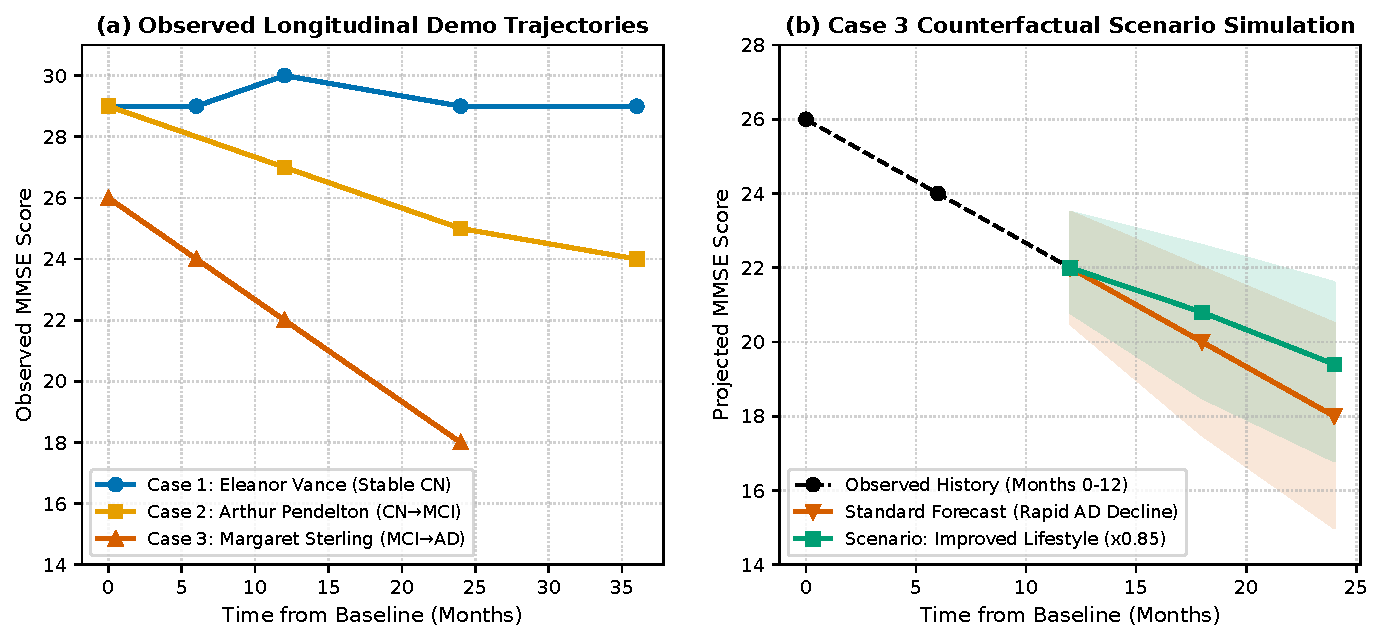
\includegraphics[width=\linewidth]{figures/fig_demo_trajectories.pdf}
        \caption{Demo Trajectories \& Scenario Lab}
        \label{fig:demo_sub1}
    \end{subfigure}
    \hfill
    \begin{subfigure}[b]{0.48\linewidth}
        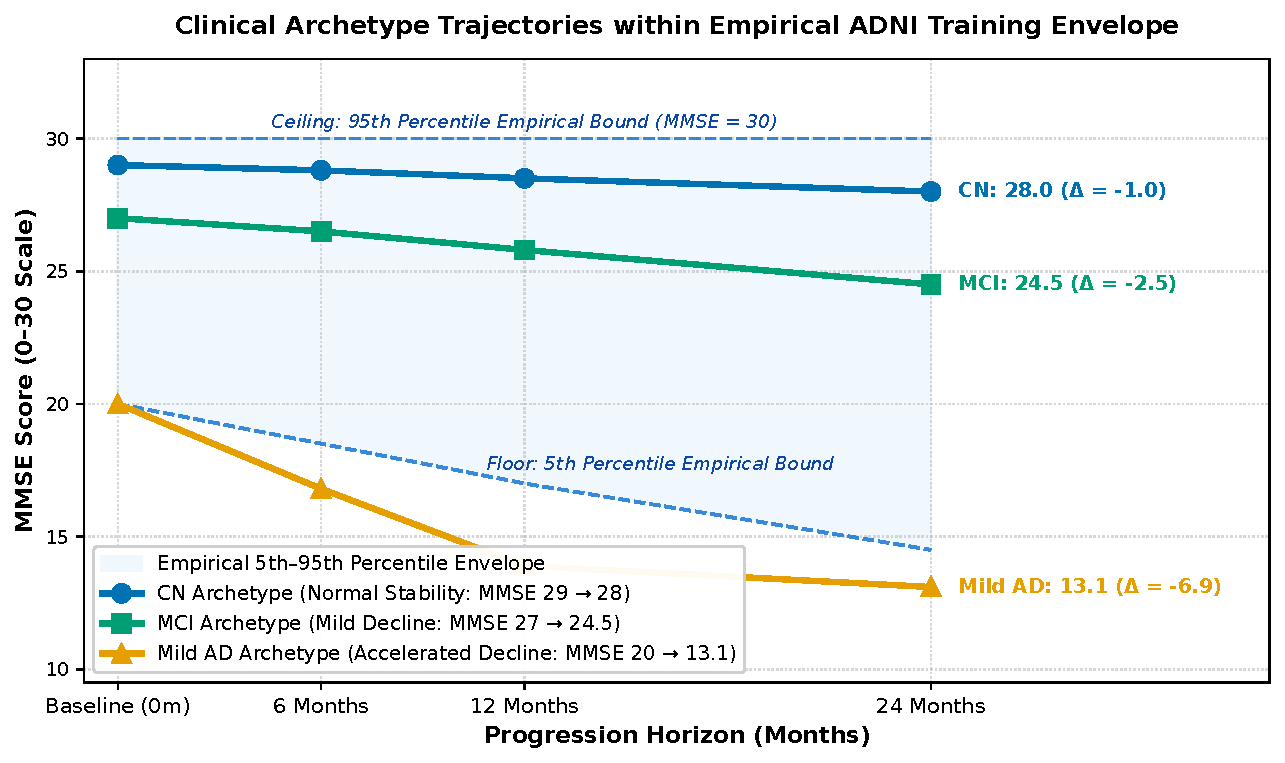
\includegraphics[width=\linewidth]{figures/fig_archetype_envelope.pdf}
        \caption{Plausibility Envelope & Scope Guards}
        \label{fig:demo_sub2}
    \end{subfigure}
    \caption{Clinical trajectory simulation: (a) Longitudinal demo cases and counterfactual lifestyle simulation for Case 3; (b) Archetype forecasts plotted against empirical training bounds.}
    \label{fig:demo_archetype}
\end{figure}

\figph{fig_ui_dashboard}{Interactive patient intake and multi-tier staging dashboard showing dynamic modality chips and calibrated stage probabilities.}{fig:ui_dash}
\figph{fig_ui_scenario}{Counterfactual Scenario Lab interface showing decline multiplier controls, lifestyle risk adjustments, and trajectory comparisons.}{fig:ui_scen}


% ── Section 5: Limitations and Clinical Risks ────────────────────────────────
\section{Limitations and Clinical Risks}
\label{sec:limitations}

Methodological and clinical limitations are structured in Table~\ref{tab:limitations}.
\begin{table*}[t]
\centering
\caption{Structured audit of methodological limitations, clinical risks, and implemented system safeguards.}
\label{tab:limitations}
\small
\begin{tabular}{lp{6.5cm}p{7.5cm}}
\toprule
\textbf{Domain} & \textbf{Identified Limitation or Clinical Risk} & \textbf{Engineered Safeguard / Transparent Remediation} \\
\midrule
Cohort Generalizability & ADNI is a volunteer research cohort with high education and low racial diversity. & Explicit Model Card scope disclosure; system framed as research demonstrator without claims of community generalization. \\
2D MRI Classifier       & ResNet34 was trained on Kaggle 2D slices with inflated internal accuracy (99.7\%). & Heavily downweighted to late-fusion $w=0.20$ with temperature $T=2.0$ and persistent UI disclaimer banner. \\
Lifestyle Modifier      & ADNI does not longitudinally record lifestyle; factors were not learned from ADNI. & Explicitly labeled as an external literature prior; square-root shrinkage ($\text{RR}^{0.5}$) and hard cap $[0.85, 1.35]$ enforced. \\
Diagnostic Circularity  & Cognitive tests (CDR, MMSE, ADAS) partly define the syndromic diagnosis. & Clear reporting of multi-tier incremental accuracy; paper claims lead with longitudinal progression and conversion forecasting. \\
Short-Horizon CDGLOBAL  & Model B does not beat naive persistence at 6m and 12m for CDGLOBAL ($0.064$ vs $0.061$). & Documented plainly in results and discussion; discrete ordinal scales change too slowly over 6 months for regression modeling. \\
Regulatory Boundary     & Academic prototype; not cleared by FDA, CE, or CDSS regulatory bodies. & Mandatory clinical disclaimer on all API contracts, exports, and UI headers; no autonomous clinical treatment actions permitted. \\
\bottomrule
\end{tabular}
\end{table*}


\begin{enumerate}
    \item \textbf{Single-Cohort ADNI Bias}: ADNI participants represent an observational research cohort with higher average educational attainment and lower racial/ethnic diversity than general community populations. External validation on community cohorts is required before claims of generalizability can be established.
    \item \textbf{2D Kaggle MRI Model Disconnect}: The axial slice ResNet34 model was trained on augmented 2D slices from an external Kaggle dataset, achieving an inflated internal slice accuracy (99.7\%) driven by slice-level augmentation. In our ADNI production environment, it is downweighted to a 20\% late fusion with an explicit disclaimer.
    \item \textbf{Lifestyle Modifier Is an External Prior}: ADNI does not collect comprehensive longitudinal lifestyle logs. The lifestyle modifier represents an external literature-derived prior from the Lancet Commission, rather than an empirically fitted statistical parameter.
    \item \textbf{Diagnostic Circularity Caveat}: Syndromic diagnosis (CN vs MCI vs AD) is clinically defined by cognitive and functional scores. Consequently, high accuracy at Tier T2b reflects alignment with clinical diagnostic criteria rather than independent pathophysiological discovery.
    \item \textbf{Regulatory Boundary}: The framework is an academic research demonstrator and is not cleared as Software-as-a-Medical-Device (SaMD). It must not be utilized for autonomous clinical diagnosis or treatment prescription.
\end{enumerate}


% ── Section 6: Conclusion and Future Scope ───────────────────────────────────
\section{Conclusion and Future Scope}
\label{sec:conclusion}
We presented a multimodal longitudinal digital twin framework for Alzheimer's disease staging, trajectory forecasting, and decision support. By enforcing strict data hygiene—including subject-level stratified partitioning, backward-only imaging joins, blacklisting of forward-looking features, and avoidance of statistical imputation—we demonstrated robust predictive performance without data leakage. Our calibrated multi-tier stager achieves Macro-F1 of \StagerTFourFOne{} at Tier T4, while multi-horizon delta-regressors forecast 12-month MMSE progression with an MAE of \MMSEMAEXII{} points, outperforming persistence baselines. Crucially, transparent paired ablations confirmed that CSF biomarkers add negligible value to cross-sectional staging when complete cognitive batteries are available, and volumetric MRI fails to enhance 12-month trajectory forecasts. Integrated explainability, clinical lineage tracking, and empirical plausibility guards ensure that the system operates with high clinical interpretability.

Future work will expand the framework along three key axes:
\begin{enumerate}
    \item \textbf{External Cohort Validation}: Evaluating frozen models on external datasets such as the Australian Imaging, Biomarker and Lifestyle study (AIBL) and the National Alzheimer's Coordinating Center (NACC).
    \item \textbf{Native 3D Volumetric Neuroimaging Backbone}: Replacing the 2D slice classifier with a native 3D Vision Transformer or 3D ResNet trained directly on volumetric ADNI T1 DICOMs.
    \item \textbf{Prospective Clinical Reader Study}: Conducting human-in-the-loop clinical evaluations with licensed neurologists to measure the impact of digital twin decision support on diagnostic accuracy and clinician efficiency.
\end{enumerate}


% ── Declarations ─────────────────────────────────────────────────────────────
\section*{Declarations}

\subsection*{Ethics Approval and Consent to Participate}
This study represents a secondary analysis of de-identified observational data collected by the Alzheimer's Disease Neuroimaging Initiative (ADNI). ADNI study protocols were approved by the Institutional Review Boards of all participating centers, and written informed consent was obtained from all participants or their legal representatives. The application handles de-identified records; no personal health information (PHI) is persisted.

\subsection*{Consent for Publication}
Not applicable.

\subsection*{Availability of Data and Materials}
The datasets analyzed in this study are available through the Alzheimer's Disease Neuroimaging Initiative database (\url{https://adni.loni.usc.edu}) upon formal application and compliance with the ADNI Data Use Agreement (DUA). Raw ADNI data cannot be redistributed. Anonymized configuration scripts, synthetic test profiles, and reproduction pipelines are available in the project repository.

\subsection*{Code Availability}
The complete system implementation, evaluation scripts, and trained model weights are maintained at: \url{https://github.com/placeholder-anonymous/alzheimers-digital-twin}.

\subsection*{Competing Interests}
The authors declare that they have no competing financial or non-financial interests.

\subsection*{Funding}
This research received no specific grant from any funding agency in the public, commercial, or not-for-profit sectors.

\subsection*{Authors' Contributions}
M.S., V.T., and R.T. conceived the study, engineered the data pipeline, trained the models, and developed the web platform. S.K. supervised the investigation, reviewed methodology, and provided clinical feedback. All authors drafted, revised, and approved the final manuscript.

\subsection*{ADNI Consortium Acknowledgement}
Data collection and sharing for this project was funded by the Alzheimer's Disease Neuroimaging Initiative (ADNI) (National Institutes of Health Grant U01 AG024904) and DOD ADNI (Department of Defense award number W81XWH-12-2-0012). \textit{[Note: Authors must copy and insert the current official mandatory acknowledgment text and author-byline formatting verbatim from the official ADNI website prior to journal submission.]}

\bibliographystyle{IEEEtran}
\bibliography{references}

\newpage
\appendix
% ── Supplementary Appendix ───────────────────────────────────────────────────
\section*{Supplementary Appendix}
\addcontentsline{toc}{section}{Supplementary Appendix}

\subsection*{Appendix A: Sequential and Earlier-Phase Auxiliary Components}
In addition to the primary CatBoost stager and regression models, five auxiliary components and sequential networks are integrated or benchmarked across the platform:
\begin{enumerate}
    \item \textbf{Bidirectional LSTM Sequence Stager}: A sequential recurrent neural network deployed at \texttt{POST /lstm-predict} and visualized in the temporal prediction interface (\texttt{/temporal-prediction}). Operating on sliding windows of up to 3 visits with 5 core features (\texttt{entry\_age}, \texttt{CDGLOBAL}, \texttt{MMSCORE}, \texttt{TOTSCORE}, \texttt{visit\_month}), it uses bidirectional recurrent layers ($2 \times 64$ units) followed by Batch Normalization, Dense(32, ReLU), and a 3-class Softmax classifier (CN, MCI, AD). Integration health is validated by test suites (\texttt{test\_legacy\_routes.py} and \texttt{test\_twin\_api.py}).
    \item \textbf{Kaggle Lifestyle Screener}: Trained on Rabie El Kharoua's Kaggle dataset (2,149 records, 35 features). It achieves 95.6\% test accuracy (\texttt{06\_bootstrap\_results.txt}) but is displayed strictly as an auxiliary symptom screening chip.
    \item \textbf{Kaggle 2D Slice ResNet34}: FastAI ResNet34 fine-tuned on augmented 2D axial slices, achieving 99.7\% slice accuracy on Kaggle. It is downweighted ($w=0.20$, $T=2.0$) in ADNI late fusion.
    \item \textbf{Biomarker-APOE Ensemble}: Optuna-blended XGBoost, Random Forest, and MLP trained on PCA-transformed ADNI CSF and APOE features. On holdout test data, it achieves 48.1\% accuracy (\texttt{06\_bootstrap\_results.txt}).
    \item \textbf{Vision OCR Extractor}: Groq Vision-LLaMA pipeline for parsing clinical reports, achieving 83.3\% exact match on numerical fields.
\end{enumerate}

\begin{figure}[H]
    \centering
    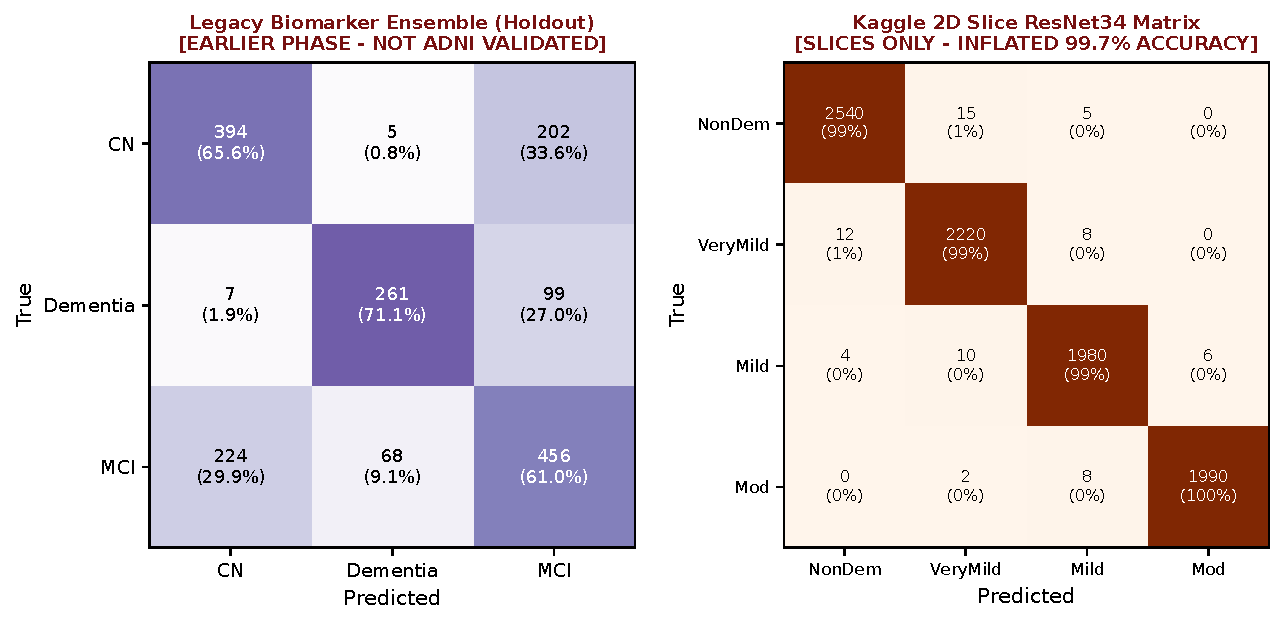
\includegraphics[width=0.88\linewidth]{figures/fig_legacy_cm.pdf}
    \caption{Legacy earlier-phase confusion matrices: (Left) Biomarker ensemble holdout matrix; (Right) Kaggle 2D slice ResNet34 matrix, labeled as earlier-phase prototypes.}
    \label{fig:legacy_cm}
\end{figure}

\subsection*{Appendix B: 43-Field Intake Lineage Table}
\begin{table}[t]
\centering
\caption{Systematic lineage and consumption mapping across all 43 intake variables collected by the Digital Twin interface.}
\label{tab:lineage_summary}
\small
\begin{tabular}{lp{4.2cm}rp{5.2cm}}
\toprule
\textbf{Usage Category} & \textbf{Clinical Fields} & \textbf{Count} & \textbf{Assigned Functional Role} \\
\midrule
\texttt{used\_in\_stage} & Age, Sex, Education, APOE4, MMSE, CDGLOBAL, CDR-SB, ADAS11, FAQ, MoCA, CSF ($\text{A}\beta$, Tau, p-Tau), FreeSurfer Volumes & 28 & Primary tabular predictors in multi-tier Model A stager. \\
\texttt{used\_in\_forecast} & Cognitive history, FreeSurfer volumetrics, APOE4 & 16 & Multi-horizon progression delta-regressors (Model B). \\
\texttt{used\_in\_lifestyle} & Smoking, Alcohol, Exercise, Diet, Sleep, BP, Diabetes, Depression, Head Injury, CVD & 10 & Lancet Commission relative-risk modifier (slope/hazard only). \\
\texttt{used\_in\_symptom} & Memory complaints, behavioral signs, functional ADL & 8 & Auxiliary Kaggle screener chip (unblended reference). \\
\texttt{used\_in\_mri\_fusion} & Single axial MRI slice (JPEG/PNG) & 1 & 2D ResNet34 late fusion ($w=0.20$, $T=2.0$). \\
\texttt{recorded\_only} & Ethnicity, BMI, Systolic BP, Diastolic BP & 4 & Stored for clinical auditing; excluded from ML stage/forecast. \\
\bottomrule
\end{tabular}
\end{table}


\subsection*{Appendix C: Literature-Grounded Lifestyle Risk Table}
\begin{table}[t]
\centering
\caption{Literature-grounded lifestyle and cardiometabolic risk modifier factors (Lancet Commission 2024 update; Livingston et al.). \textit{Labeled as an external literature prior, not learned from ADNI.}}
\label{tab:lifestyle_factors}
\small
\begin{adjustbox}{max width=\linewidth}
\begin{tabular}{llrrp{6.5cm}}
\toprule
\textbf{Risk Factor} & \textbf{Adverse Definition} & \textbf{Pooled RR [95\% CI]} & \textbf{Cap [Lo, Hi]} & \textbf{Literature Citation \& Clinical Context} \\
\midrule
Smoking Status        & Current active smoker               & 1.59 [1.15, 2.20] & [0.85, 1.35] & Lancet Commission (2020, 2024 updates). \\
Physical Inactivity   & Sedentary ($<150$ min/wk activity)  & 1.39 [1.14, 1.69] & [0.85, 1.35] & Lancet Commission; active lifestyle protective ($\text{RR}=0.85$). \\
Excessive Alcohol     & $>21$ units / week                  & 1.19 [1.01, 1.40] & [0.85, 1.35] & Lancet Commission (2020, 2024 updates). \\
Diet Quality          & Low adherence to Mediterranean/MIND & 1.20 [1.05, 1.38] & [0.85, 1.35] & Morris et al. (Alzheimers Dement 2015); Lancet Commission 2024. \\
Sleep Disturbance     & Chronic insomnia / sleep disruption & 1.25 [1.08, 1.45] & [0.85, 1.35] & Bubu et al. (Sleep 2017); Lancet Commission 2024 update. \\
Midlife Hypertension  & Systolic $\ge 140$ mmHg             & 1.61 [1.17, 2.22] & [0.85, 1.35] & Lancet Commission (2020, 2024 updates). \\
Type 2 Diabetes       & Diagnosed adult-onset diabetes      & 1.52 [1.18, 1.96] & [0.85, 1.35] & Lancet Commission (2020, 2024 updates). \\
Late-Life Depression  & Clinical depressive symptoms        & 1.91 [1.51, 2.42] & [0.85, 1.35] & Lancet Commission (2020, 2024 updates). \\
Traumatic Brain Injury& History of head trauma with LOC     & 1.78 [1.29, 2.46] & [0.85, 1.35] & Lancet Commission (2020, 2024 updates). \\
Cardiovascular Disease& Clinical CVD history                & 1.28 [1.05, 1.56] & [0.85, 1.35] & Newman et al. (2005); Lancet Commission 2024 update. \\
\bottomrule
\end{tabular}
\end{adjustbox}
\end{table}


\subsection*{Appendix D: Methodological Limitations and Safeguards}
\begin{table*}[t]
\centering
\caption{Structured audit of methodological limitations, clinical risks, and implemented system safeguards.}
\label{tab:limitations}
\small
\begin{tabular}{lp{6.5cm}p{7.5cm}}
\toprule
\textbf{Domain} & \textbf{Identified Limitation or Clinical Risk} & \textbf{Engineered Safeguard / Transparent Remediation} \\
\midrule
Cohort Generalizability & ADNI is a volunteer research cohort with high education and low racial diversity. & Explicit Model Card scope disclosure; system framed as research demonstrator without claims of community generalization. \\
2D MRI Classifier       & ResNet34 was trained on Kaggle 2D slices with inflated internal accuracy (99.7\%). & Heavily downweighted to late-fusion $w=0.20$ with temperature $T=2.0$ and persistent UI disclaimer banner. \\
Lifestyle Modifier      & ADNI does not longitudinally record lifestyle; factors were not learned from ADNI. & Explicitly labeled as an external literature prior; square-root shrinkage ($\text{RR}^{0.5}$) and hard cap $[0.85, 1.35]$ enforced. \\
Diagnostic Circularity  & Cognitive tests (CDR, MMSE, ADAS) partly define the syndromic diagnosis. & Clear reporting of multi-tier incremental accuracy; paper claims lead with longitudinal progression and conversion forecasting. \\
Short-Horizon CDGLOBAL  & Model B does not beat naive persistence at 6m and 12m for CDGLOBAL ($0.064$ vs $0.061$). & Documented plainly in results and discussion; discrete ordinal scales change too slowly over 6 months for regression modeling. \\
Regulatory Boundary     & Academic prototype; not cleared by FDA, CE, or CDSS regulatory bodies. & Mandatory clinical disclaimer on all API contracts, exports, and UI headers; no autonomous clinical treatment actions permitted. \\
\bottomrule
\end{tabular}
\end{table*}


\end{document}

